\documentclass[ruler]{CUP-JNL-EDS}%%option ruler --> print line number in the margin


%%%% Packages
\usepackage{latexsym}
\usepackage{graphicx}
\usepackage{multicol,multirow}
\usepackage{amsmath,amssymb,amsfonts}
\usepackage{mathrsfs}
\usepackage{amsthm}
\usepackage{rotating}
\usepackage{appendix}
\usepackage{subcaption}
\usepackage[authoryear]{natbib}
\usepackage{ifpdf}
\usepackage[T1]{fontenc}
\usepackage{times}
%\usepackage{sourcesanspro}
\usepackage{newtxmath}
\usepackage{textcomp}%
\usepackage{xcolor}%
\usepackage{hyperref}
\usepackage{lipsum}
\usepackage{float}
\usepackage{algorithm}
\usepackage{algpseudocode}
%%%%

\articletype{APPLICATION PAPER}
\jname{Environmental Data Science}
%\artid{20}
\jyear{2025}
\jvol{4}
%\jissue{1}
\jdoi{10.1017/eds.2025.xx}
%\raggedbottom


\begin{document}
\begin{Frontmatter}

\title[Article Title]{Coupling Uncertainty-Aware Flow Forecasts with Policy Optimisation in Water Management}
\author[1]{Dami Akinniyi}
\address[1]{\orgdiv{Data Science Program}, \orgname{Government of Manitoba}, \orgaddress{\city{Winnipeg}, \state{MB},  \country{Canada}}}

\received{31 January 2020}
\revised{01 May 2020}
\accepted{06 May 2020}

\authormark{Akinniyi, D.}

\keywords{ Calibrated Ensemble Forecasting; Spatiotemporal Modelling, Gradient Boosting Trees, Policy Synthesis, Evolutionary Optimisation}

\abstract{This paper presents the 1st place entry to the Capgemini Invent Water Scarcity Hackathon, 
demonstrating an application that couples uncertainty-aware flow forecasting with adaptive policy 
optimization in water management. The forecasting framework integrates feature selection strategies 
with gradient boosting trees to identify and quantify the influence of dynamic and static streamflow 
drivers. By incorporating causal structure and mutual information regression for feature selection, 
the approach supports robust spatiotemporal generalization while accounting for uncertainty through 
group-bounded conformal calibration.

In parallel, policy functions were designed and optimized in a multi-objective setting to balance 
ecological and economic trade-offs under resource scarcity. The optimization framework explores the 
impact of quotas and incentive mechanisms on system outcomes, showing how prioritizing specific actors 
can intensify ecological stress and economic imbalance, while subsidies encourage cooperation but risk 
undermining resilience in highly stressed environments. By contrast, adaptive and well-calibrated policies 
promote ecofairness, ecological survival, and system stability under uncertainty.

This application illustrates how spatiotemporally generalizable, uncertainty-aware forecasts and adaptive 
policy design can together inform resilient strategies for sustainable water management.}

\policy{This application paper demonstrates a framework for uncertainty-aware water management under scarcity. 
Streamflow forecasts are generated using chained quantile regression, with \textit{k} k-means clustering applied to 
group spatial locations for calibration and reduce predictive uncertainty. Separately, quota- and 
incentive-based policy functions are optimized in a multi-objective framework to balance ecological resilience 
and economic benefit. This framework illustrates how data-driven forecasting and policy optimization can support 
robust decision-making in real-world water management scenarios.}

\end{Frontmatter}


\section{Flow Forecasting}
The first section focuses on building models to forecast water flow at stations on river basins in 
France (Adour-Garonne, Rhône-Mediterranean) and Brazil (Doce River). It involved 
predicting streamflow four weeks ahead using a combination of historical streamflow, 
observed weather, and short-term weather forecasts.\\ 

Traditional hydrological models, while effective, are often region-specific and computationally intensive, 
limiting their scalability and transferability across different catchments \citep{beven2012rainfall,singh1995}. 
In contrast, machine learning approaches leverage rich datasets with lagged and contextual features to 
capture complex temporal and spatial patterns, providing flexibility and predictive power across diverse 
hydrological settings \citep{mosavi2018, kratzert2019}. My approach builds on this paradigm by using gradient boosting 
trees \citep{prokhorenkova2018} combined with chained multi-output regression \citep{spyromitros2016} to model the spatio-temporal nature of streamflow forecasting, explicitly accounting for dependencies across 
multiple future time steps. \\

The rest of this project details the data exploration, causal analysis to identify drivers of streamflow, 
feature engineering, and modeling strategies tailored to handle differing dynamics across locations. 
It concludes with an evaluation of model performance and reflections on lessons learned for building 
robust, interpretable streamflow forecasting models.

\subsection{Related Work}
Conformal quantile calibration provides finite-sample guarantees for prediction intervals ensuring 
that the true outcome falls within the interval with a specified probability \citep{romano2019}.
However, global calibration can be inefficient in heterogeneous data, producing overly wide or 
under-confident intervals \citep{angebates2022}. This motivates approaches that calibrate within 
homogeneous groups, improving both efficiency and interpretability of predictive uncertainty.

\subsubsection*{Clustered and Class-Conditional Conformal Prediction}
Several recent works have explored calibration within homogeneous clusters to address heterogeneity. \citet{sousa2022} 
introduced an enhancement to conformalized quantile regression by incorporating k-means clustering based on feature relevance. 
This approach applies conformal steps within each cluster, allowing for adaptive prediction intervals that better 
account for heteroscedasticity. \citet{hjort2024} proposed clustered conformal prediction, grouping data points with similar 
nonconformity scores for cluster-level calibration. \citet{ding2023} extended the concept to class-conditional conformal 
prediction, clustering classes with similar conformal scores to provide accurate coverage in problems with many classes. 
These methods demonstrate that clustered calibration—based on spatial, feature, or class similarity—enhances both 
reliability and interpretability of predictive uncertainty in heterogeneous settings.

\subsubsection*{Modular Conformal Calibration (MCC)}
Modular Conformal Calibration (MCC) provides a flexible framework for recalibrating probabilistic forecasts 
from any base model by decomposing the calibration into modular components \citep{marx2022}. Each module 
targets a specific source of variability, such as temporal trends, spatial heterogeneity, or feature-dependent 
differences. By adjusting nonconformity scores independently in each module, MCC produces calibrated prediction 
intervals that are more accurate and interpretable than global calibration alone. Its generality makes it 
applicable to a wide range of models and datasets, allowing fine-grained control over the calibration process.

\subsubsection*{Adaptive Conformal Regression with Jackknife+ Rescaled Scores}
Adaptive Conformal Regression methods, such as Jackknife+ with rescaled scores, adjust nonconformity scores based 
on the magnitude of predictions and local variability. This approach ensures that intervals are appropriately wide 
where uncertainty is high and narrower where the model is more confident, improving efficiency and coverage under 
heteroscedastic data \citep{deutschmann2023}.\\

Building on these ideas, we applied relative conformal calibration (RCC) by expressing nonconformity scores relative to predicted 
values and calibrating them within spatially homogeneous groups identified via k-means clustering. This approach 
produces locally scaled, interpretable, and robust prediction intervals, ensuring reliable uncertainty estimates 
for spatiotemporally heterogeneous streamflow forecasts.

\subsection{Data Description}
\subsubsection*{Dataset Overview}
The dataset is also organized in three main splits - train, evaluation and mini challenge sets, 
to support both temporal and spatio-temporal generalization tasks. The training set is used to train the
model on historical data. The evaluation and mini-challenge sets consists of unseen temporal and Spatiotemporal
stations to evaluate the model's performance on the public leaderboard.

% \renewcommand{\arraystretch}{1.5}
\begin{table}[ht]
\centering
\begin{tabular}{llllcc}
    \hline
    \textbf{Dataset Split} & \textbf{Country} & \textbf{Coverage} & \textbf{Num\_Stations} & \textbf{Temporal} & \textbf{Spatiotemporal} \\ \hline
    Training        & France, Brazil & 1990--2003     & 39  & \checkmark & \\ 
    Evaluation      & France, Brazil & 2004--2009     & 52 - (13 new) & \checkmark & \checkmark \\ 
    Mini-challenge  & Brazil         & 2011--2015     & 2   &  & \checkmark \\ \hline
\end{tabular}
\caption{Dataset Structure and Coverage Summary}
\label{tab:station_coverage}
\end{table}
\noindent This setup poses two main challenges: temporal robustness across seen stations 
and generalization to unseen ones. This project addresses these through rigorous feature 
analysis, thoughtful feature selection, and the incorporation of causal effects to 
support reliable and responsive forecasting.

\subsubsection*{Dataset Structure}
To simulate differing hydrological conditions, the test data is comprised of a 4-week historical dataset (streamflow and weather), a 1-week weather forecast, and 
a 4-week streamflow prediction, all segmented to reflect different hydrological conditions
\begin{figure}[htbp]
    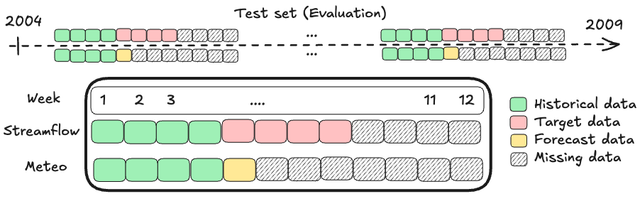
\includegraphics[width=1.0\textwidth]{./assets/images/test-set-explained.png}
    \caption{Test Set Structure}
    \label{fig:test_set_distribution}
\end{figure} 

\subsubsection*{Hydrographic Context}
\begin{figure}[htbp]
    \centering
    \begin{subfigure}[b]{1.0\textwidth}
        \centering
        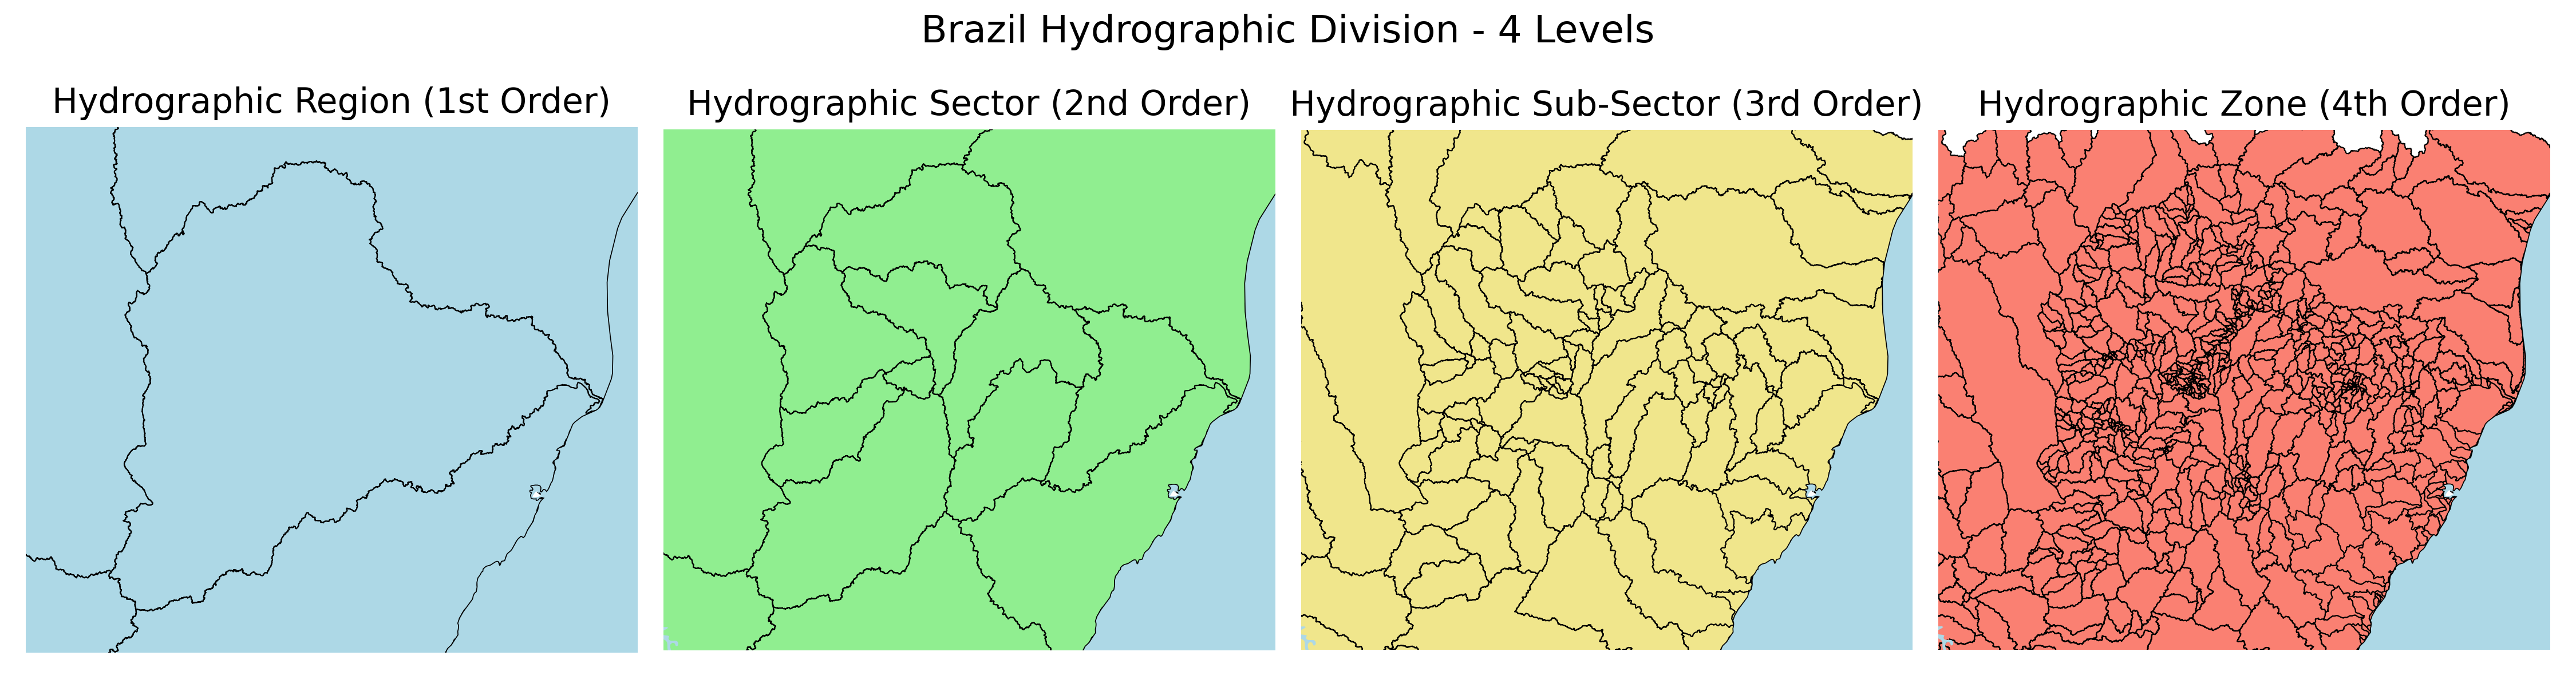
\includegraphics[width=\textwidth]{./assets/images/brazil_hydrographic_levels.png}
        \caption{Brazil}
        \label{fig:brazil_hydrographic_levels}
    \end{subfigure}
    \begin{subfigure}[b]{1.0\textwidth}
        \centering
        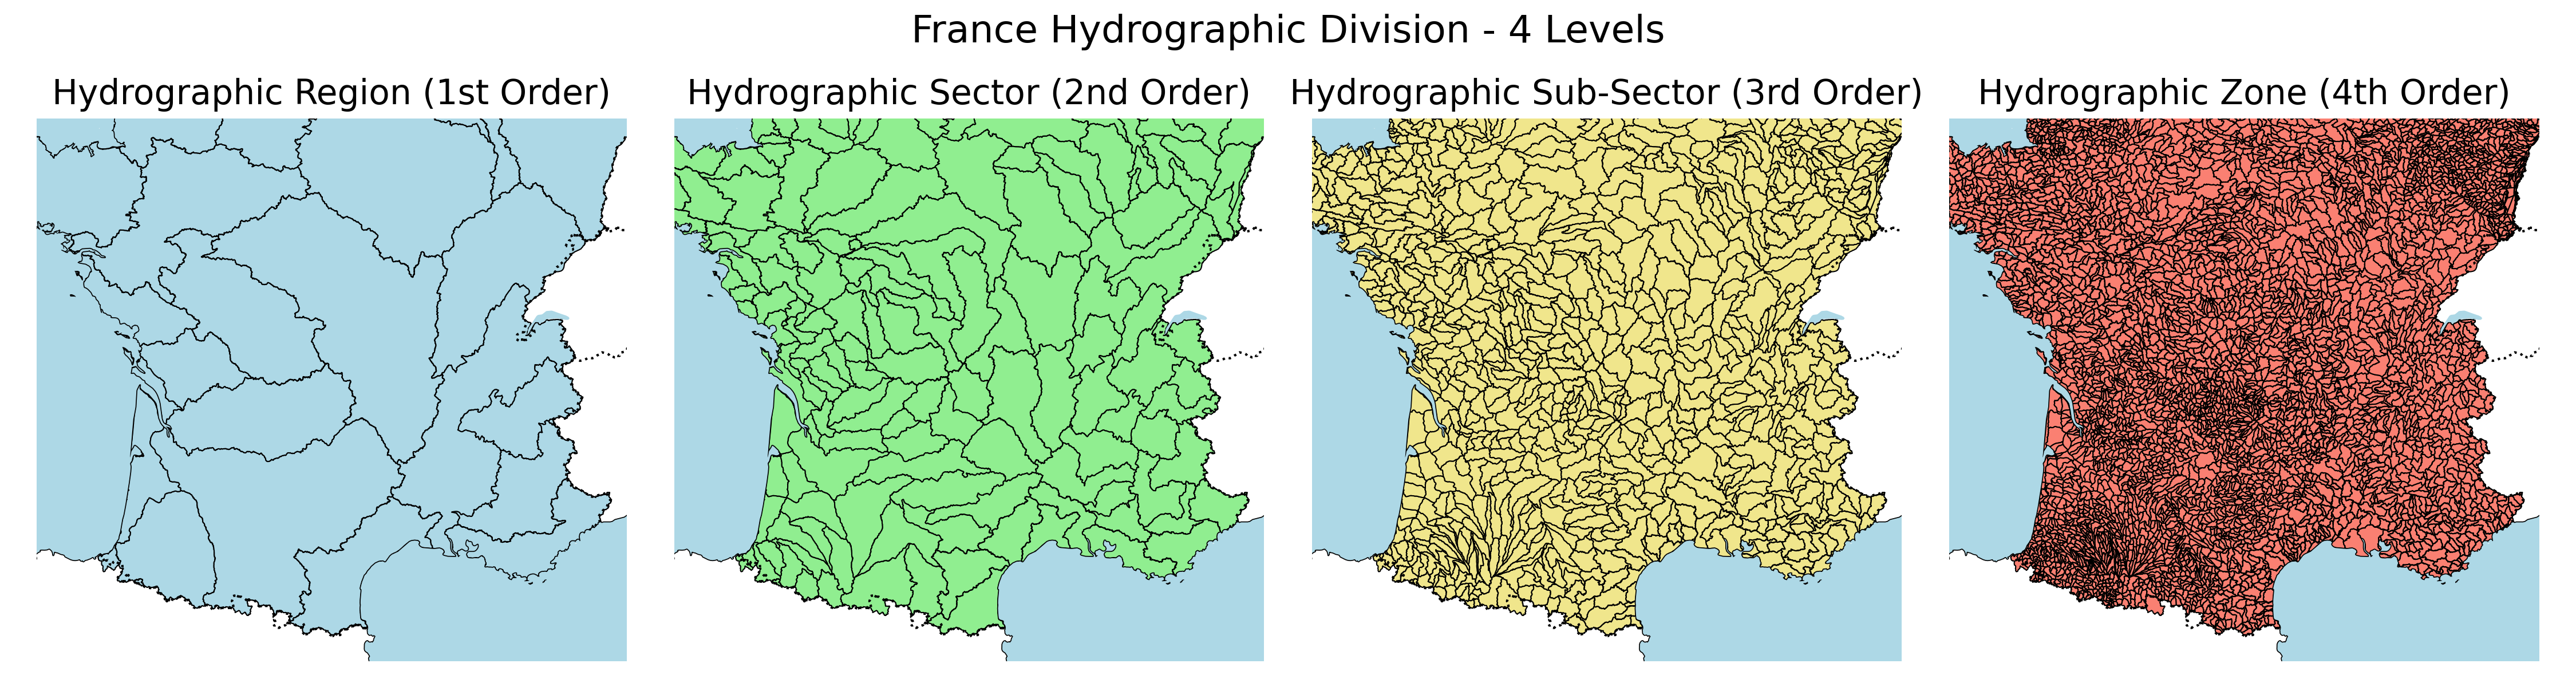
\includegraphics[width=\textwidth]{./assets/images/france_hydrographic_levels.png}
        \caption{France}
        \label{fig:france_hydrographic_levels}
    \end{subfigure}
    \caption{Spatial delineation of hydrological areas in Brazil (top) and France (bottom), across four hierarchical geoscales: region, sector, sub-sector, and zone.}
    \label{fig:hydrographic_levels_combined}
\end{figure}
The stations in both locations (Brazil and France) are distributed within hydrographic 
areas that are defined hierarchically as \textit{region, sector, sub-sector, and zone} 
(Figure \ref{fig:hydrographic_levels_combined}). Regions and sectors vary widely in land area across the two countries, sub-sectors 
and zones exhibit greater spatial consistency, making them ideal for spatial feature 
aggregation. 

\begin{figure}[htbp]
    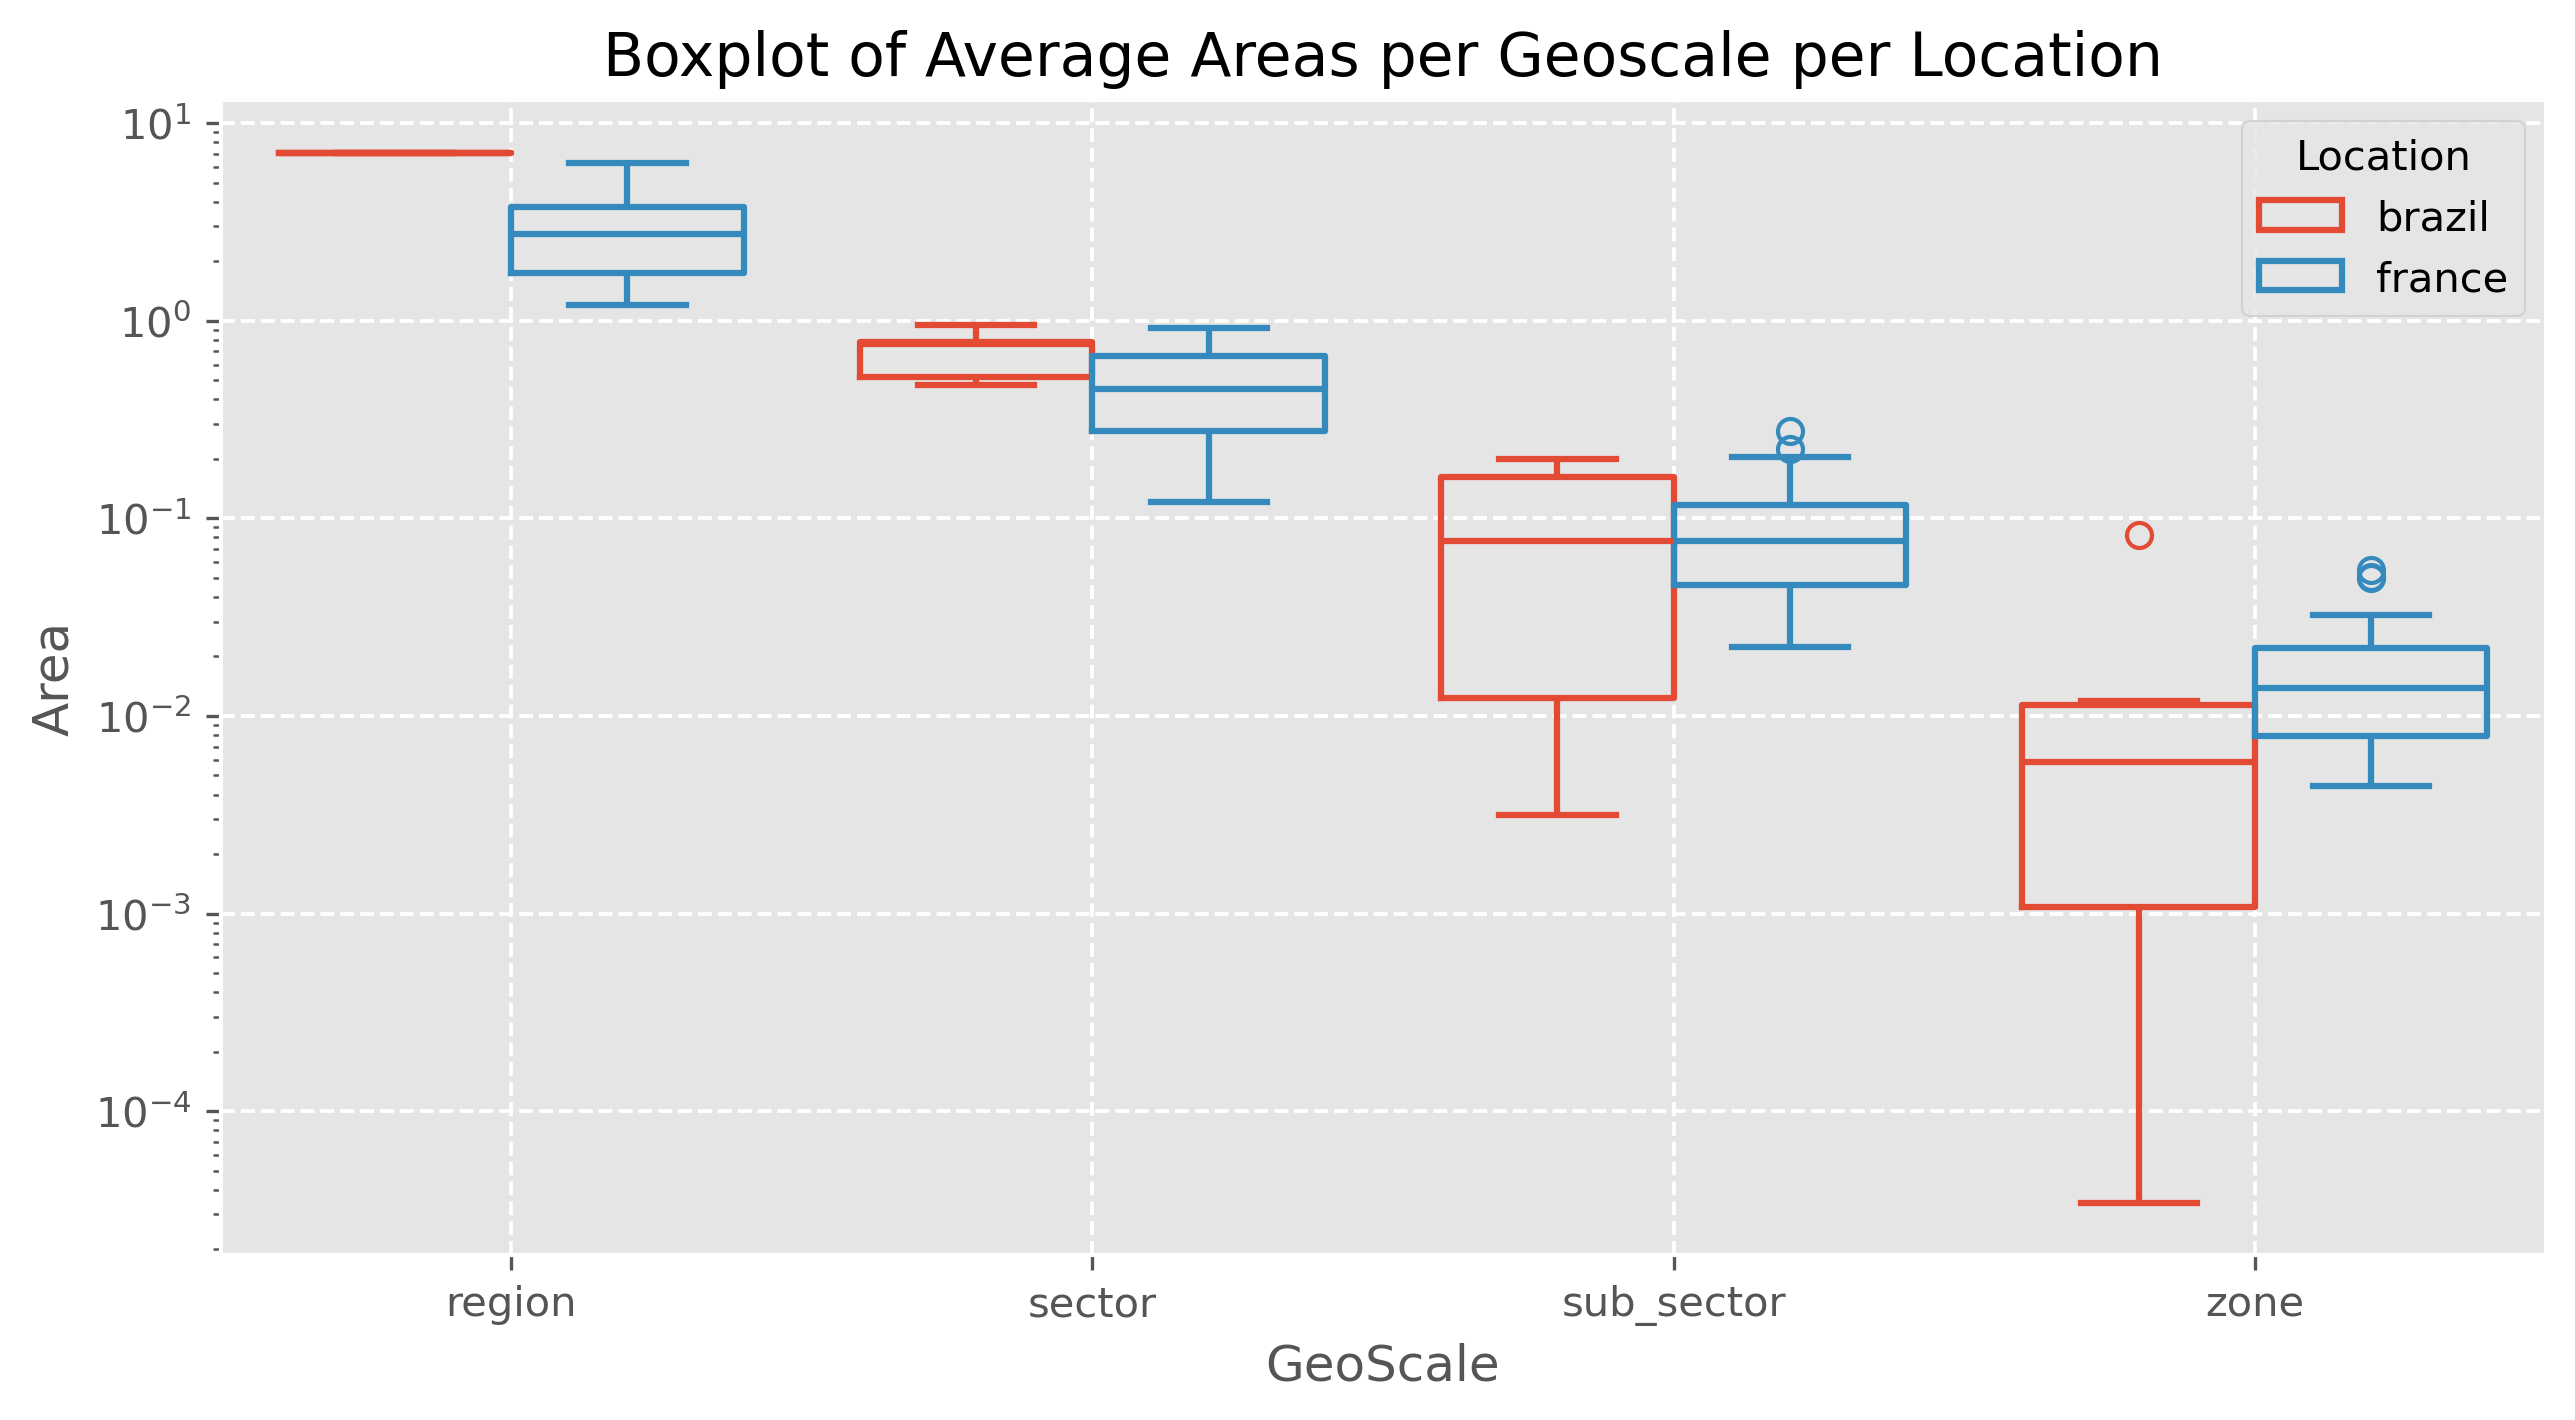
\includegraphics[width=1.0\textwidth]{./assets/images/Boxplot of Average Areas per Geoscale per Location.png}
    \caption{Boxplot comparing areas in the four geoscales in Brazil and France. The maps illustrate spatial variation in size and structure across regions, sectors, sub-sectors, and zones, highlighting differences in spatial consistency between the two countries.}
    \label{fig:geoscale_averages_per_location}
\end{figure} 

\subsubsection{Available Features}
The dataset includes a rich set of static (non-temporal) and dynamic features that capture both spatio-temporal variability in hydrological conditions.
\begin{itemize}
    \item \textbf{Static Features}: 
    \begin{itemize}
        \item Location features: Latitude, Longitude, Altitude  
        \item Hydrographic features: Region, Sector, Sub-sector, Zone, River Rank, Watershed Area  
        \item Soil composition
    \end{itemize}
    \item \textbf{Dynamic Features}: 
    \begin{itemize}
        \item Historical Streamflow
        \item Meteorological: Temperature (2m), total precipitation, evaporation, and soil moisture features 
    \end{itemize}
\end{itemize}

\subsection{Methods and Approach} 
This project follows a structured but iterative process: data preprocessing, feature engineering, 
followed by data exploration and causal analysis and finally feature selection, modelling experiments and evalutaion.
This goal at all steps preceding the modelling phase is to uncover the most relevant features for predictive accuracy,
while also ensuring that the model is interpretable and robust. The modelling phase focuses on iteratively testing different 
architectures and hyperparameters to find the best performing model.

\begin{figure}[htbp]
    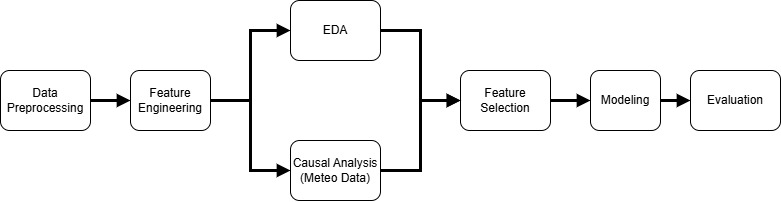
\includegraphics[width=0.9\textwidth]{./assets/method.jpg}
    \caption{Process Diagram}
    \label{fig:process_diagram}
\end{figure}

\subsubsection{Data Preprocessing}
Data preprocessing builds on the initial notebook provided in the Competition's Phase 1 GitHub repository 
which preprocesses soil and meteorological data for each station at the hydrological spatial scale. We extent 
this workflow to consolidate and structure information from multiple data sources for downstream modeling by:

\begin{itemize}
    \item integrating local spatial aggregation scales - 50km and 100km buffer scales
    \item sampling directly from xarray files for soil and meteorological data. This skips the spatial
    interpolation step in the original notebook. 
    \item modularizing and organizing all data preprocessing (for train, eval and mini-challenge) 
    into executable scripts orchestrated by a Makefile pipeline for reproducibility and scalability.
\end{itemize} 

\subsubsection{Exploratory Data Analysis}
We review the main feature groups to understand their distributions, variability, and potential predictive power.

\begin{itemize}
    \item{\textbf{Location Based Features}}: Location features, (Latitude, Longitude, Altitude), are spatially diverse 
    and capture distinct geographic patterns across regions (Figure \ref{fig:location_based_features}). These features 
    support location-aware modeling,  and enhance generalization across spatial contexts. They provide a foundation for 
    learning region-specific hydrological behavior, and are suitable proxies for such homogenous soil features 
    \citep{arsenault2023}.
    \begin{figure}[htbp]
        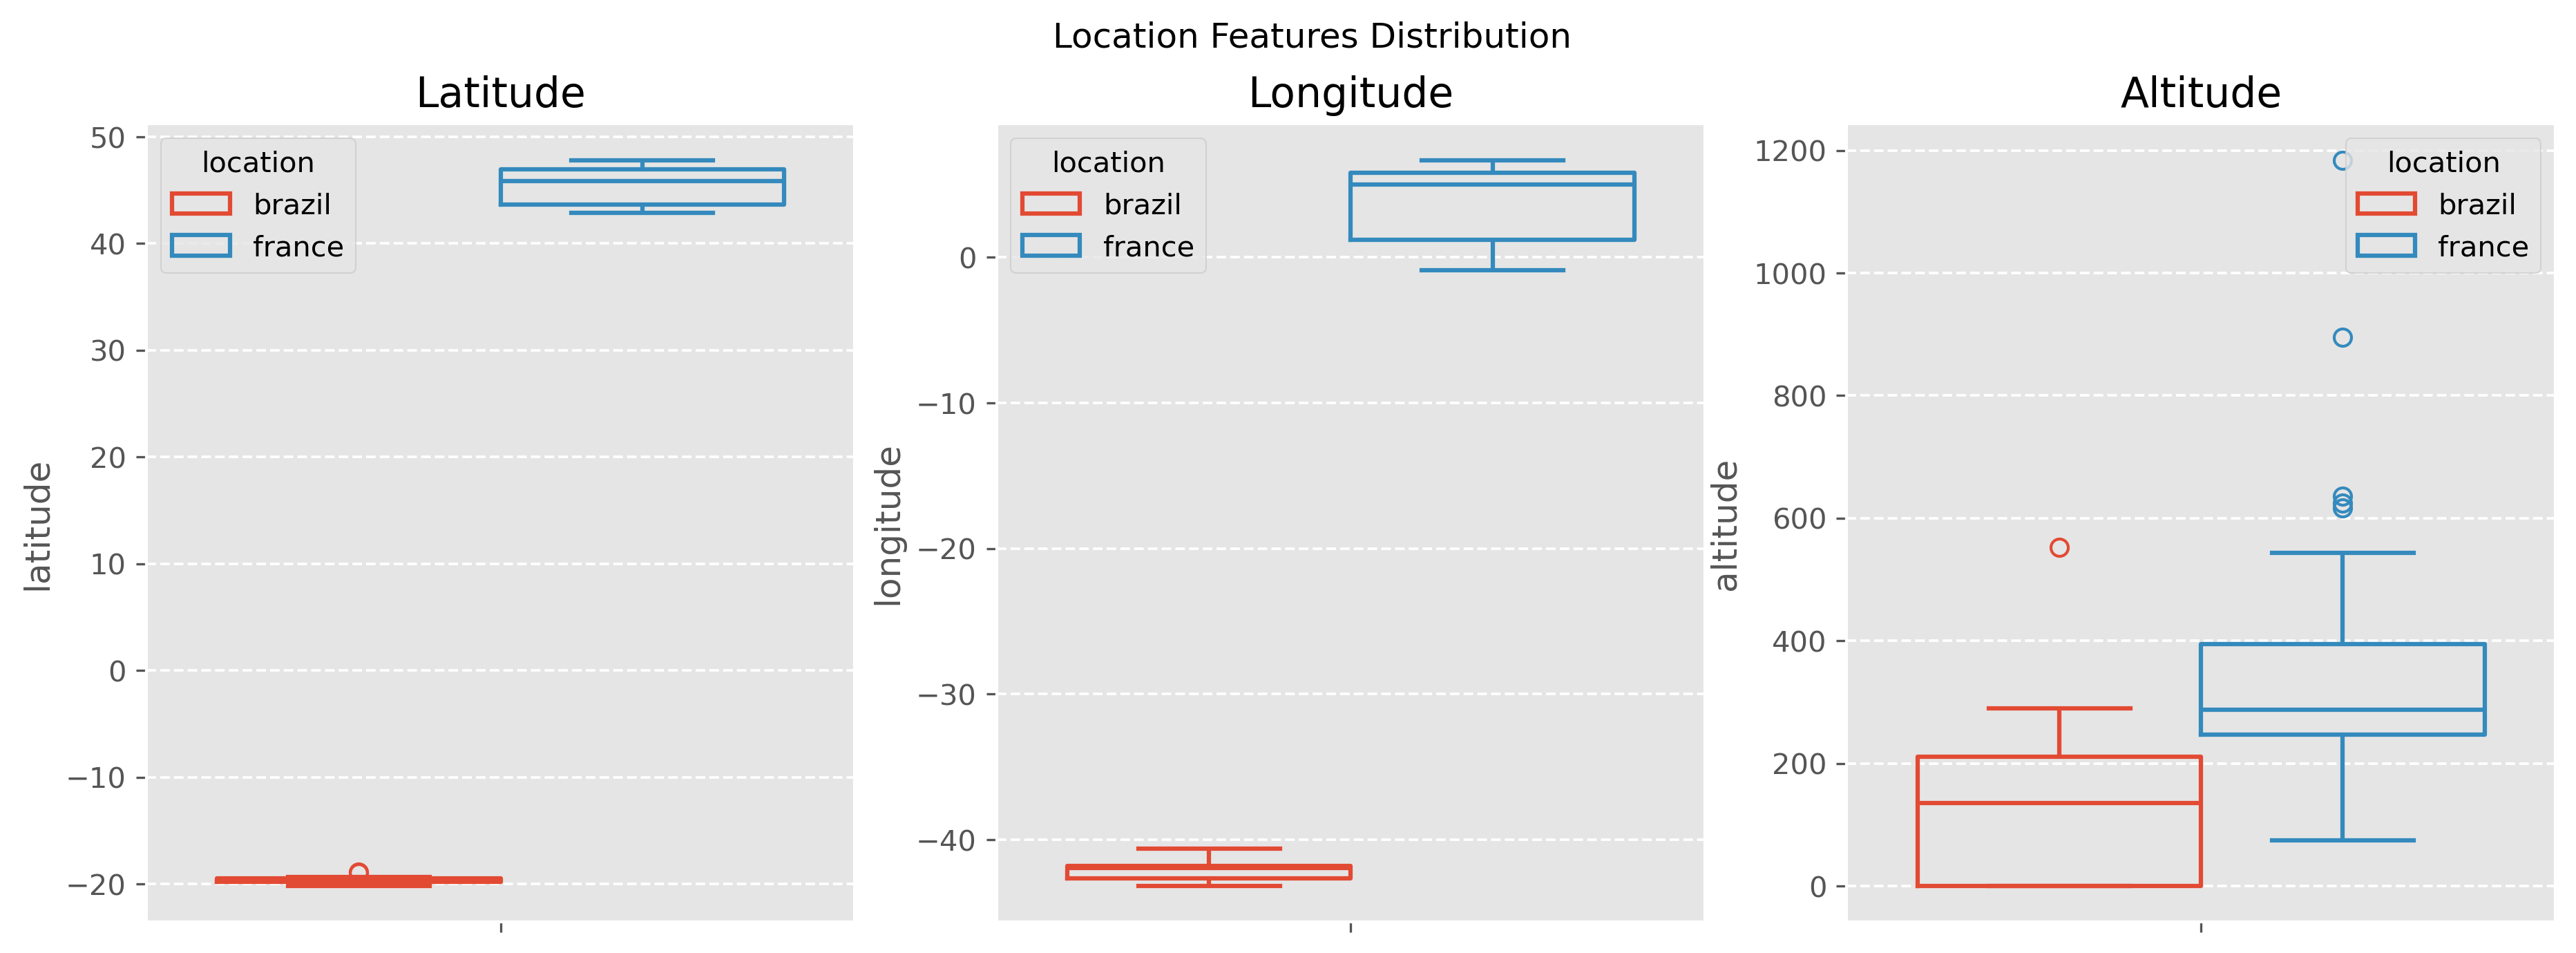
\includegraphics[width=1.0\textwidth]{./assets/images/location_features_distribution.png}
        \caption{Location-based features across the two countries.}
        \label{fig:location_based_features}
    \end{figure}
    \vspace{3mm}

    \item{\textbf{Soil Features}}: Soil features are static, with no temporal variability, limiting usage to 
    spatial modeling. This project builds on the soil aggregation methodology in the starter preprocessing notebook 
    by extending soil aggregation to incorporate both hydrological scales and buffer zones around 
    each station, enabling a multi-scale spatial understanding of soil properties. For each soil feature 
    layer, both mean values and standard deviations were computed to assess variation across depth levels 
    and geospatial units.\\ 
    The mean values within soil feature groups were generally consistent across depths and geoscales, 
    indicating minimal variation in average soil characteristics. However, standard deviations 
    showed greater variability, particularly in the upper soil layers and at the sector scale (Figure \ref{fig:soil_feature_profile}). 
    These patterns were consistent across both regions, underscoring the need for careful feature
    selection to seperate discriminative features from noisy ones.\\
    \begin{figure}[!htbp]
        \centering
        \begin{subfigure}[h]{1.0\textwidth}
            \centering
            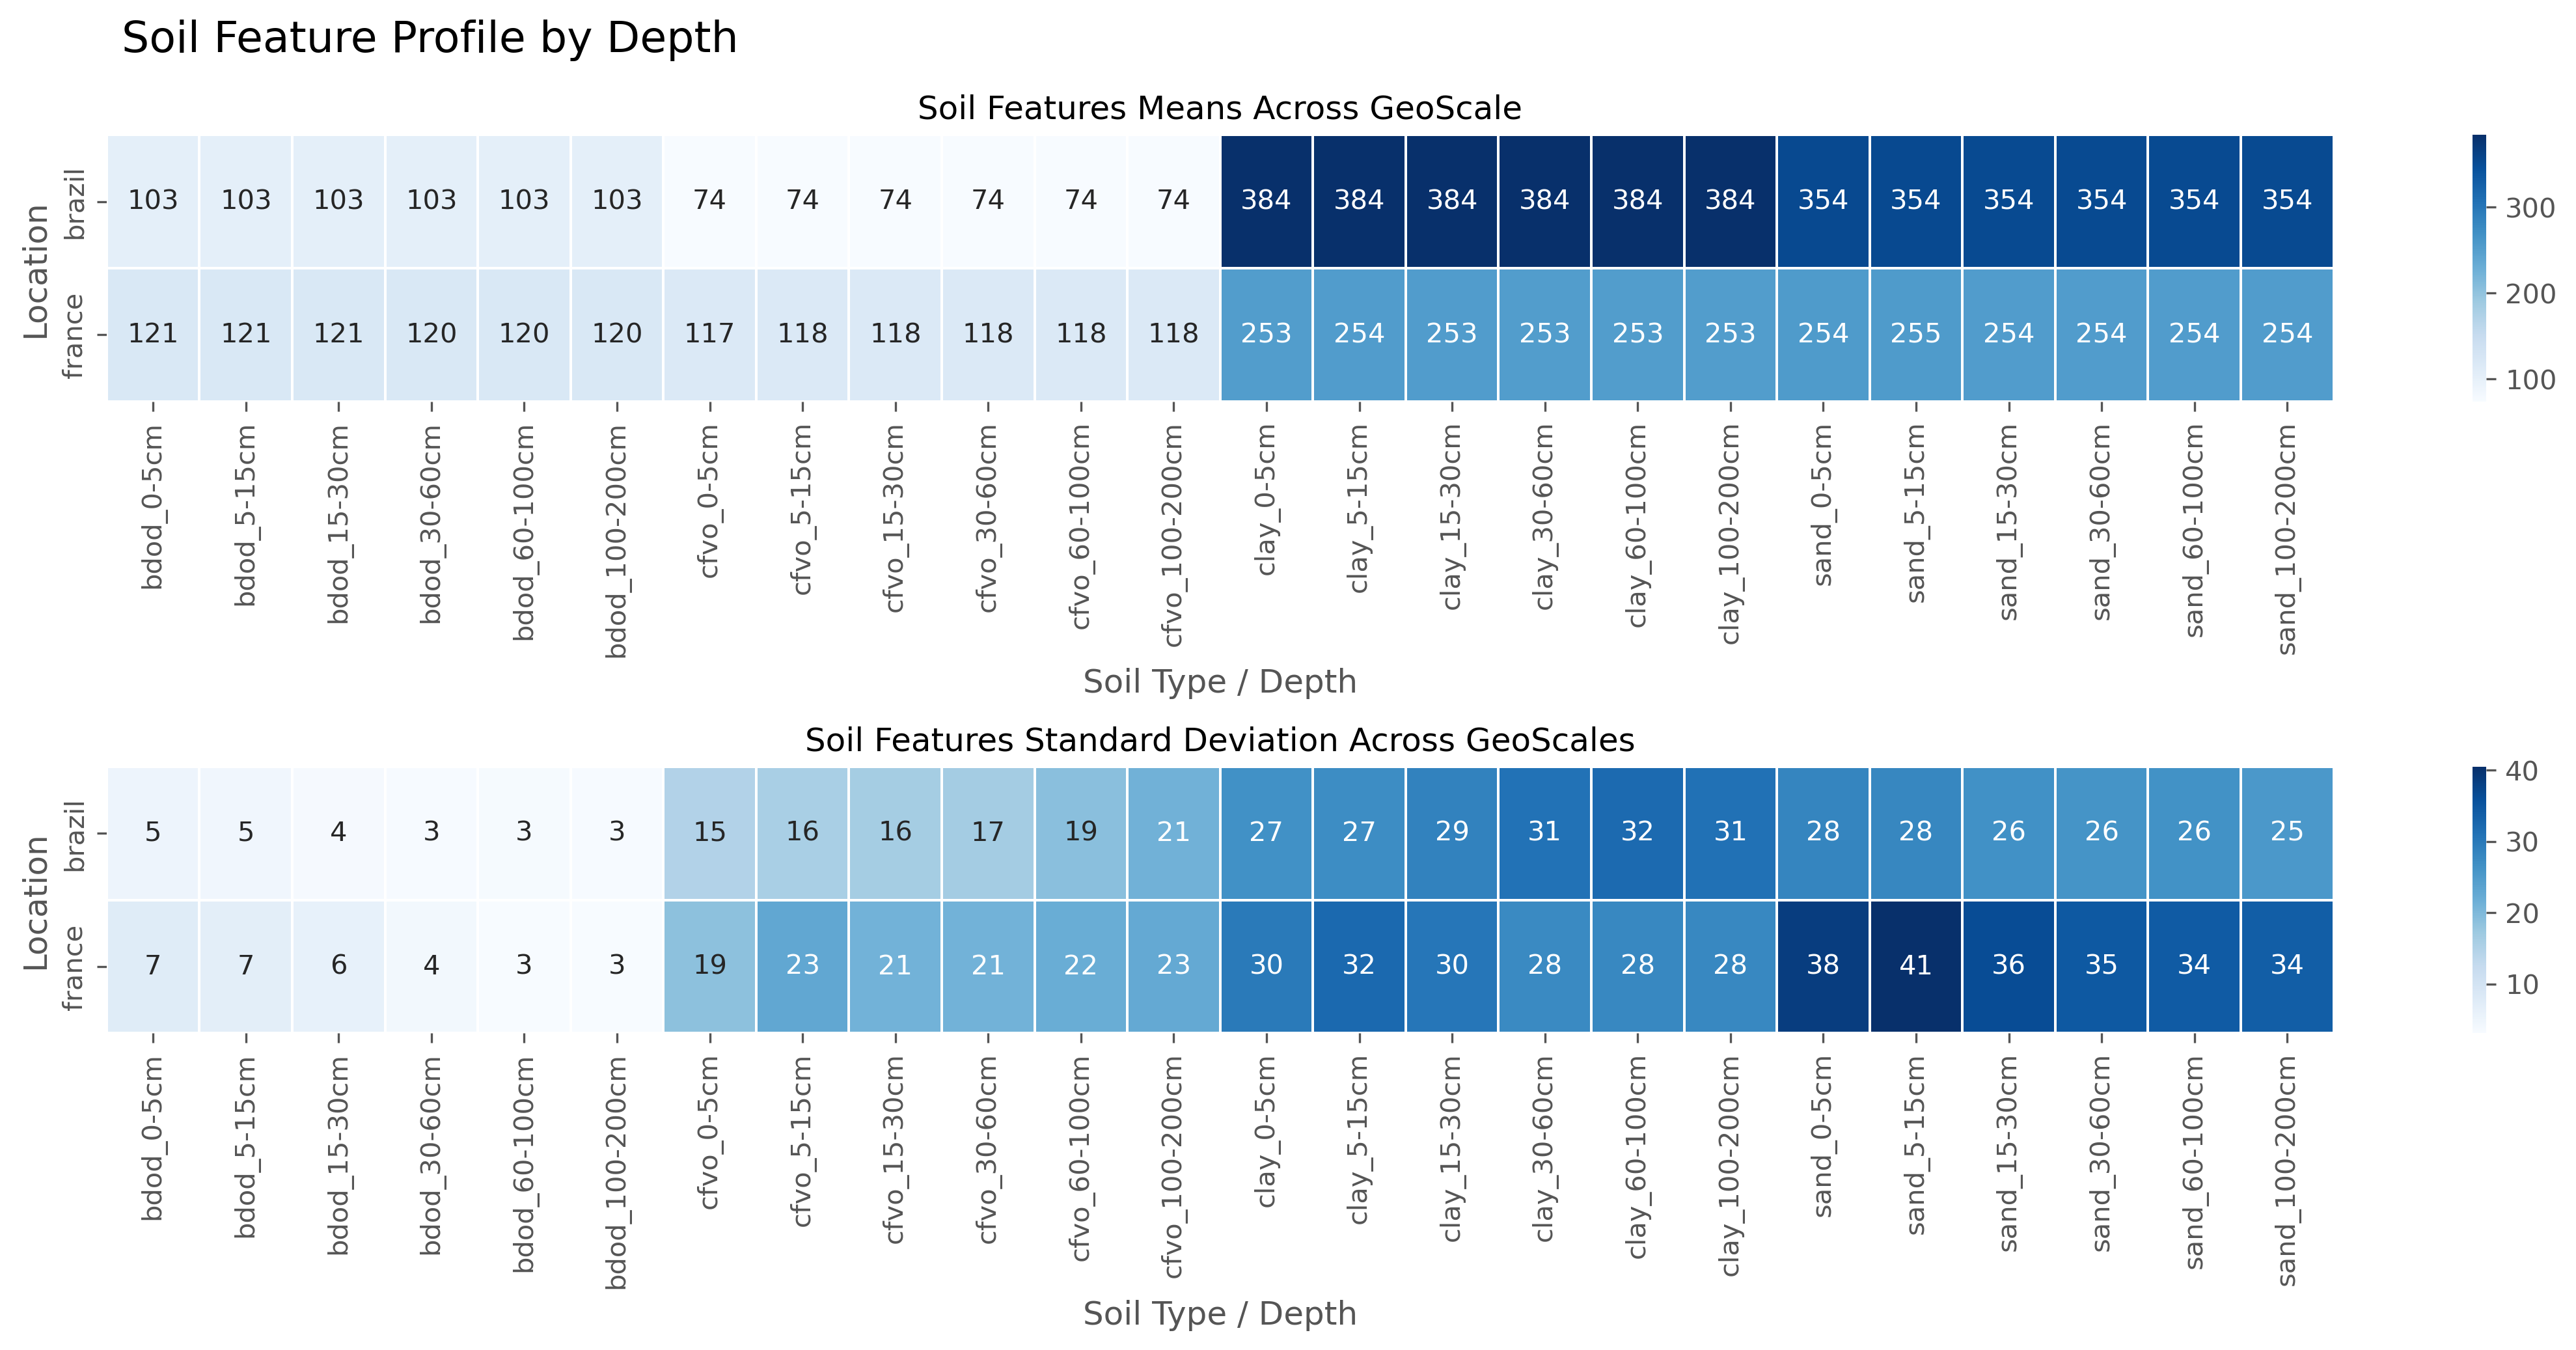
\includegraphics[width=\textwidth]{./assets/images/soil_feature_profile_depth.png}
            \caption{Soil Depth Profile}
            \label{fig:soil_feature_profile_depth}
        \end{subfigure}

        \begin{subfigure}[h]{1.0\textwidth}
            \centering
            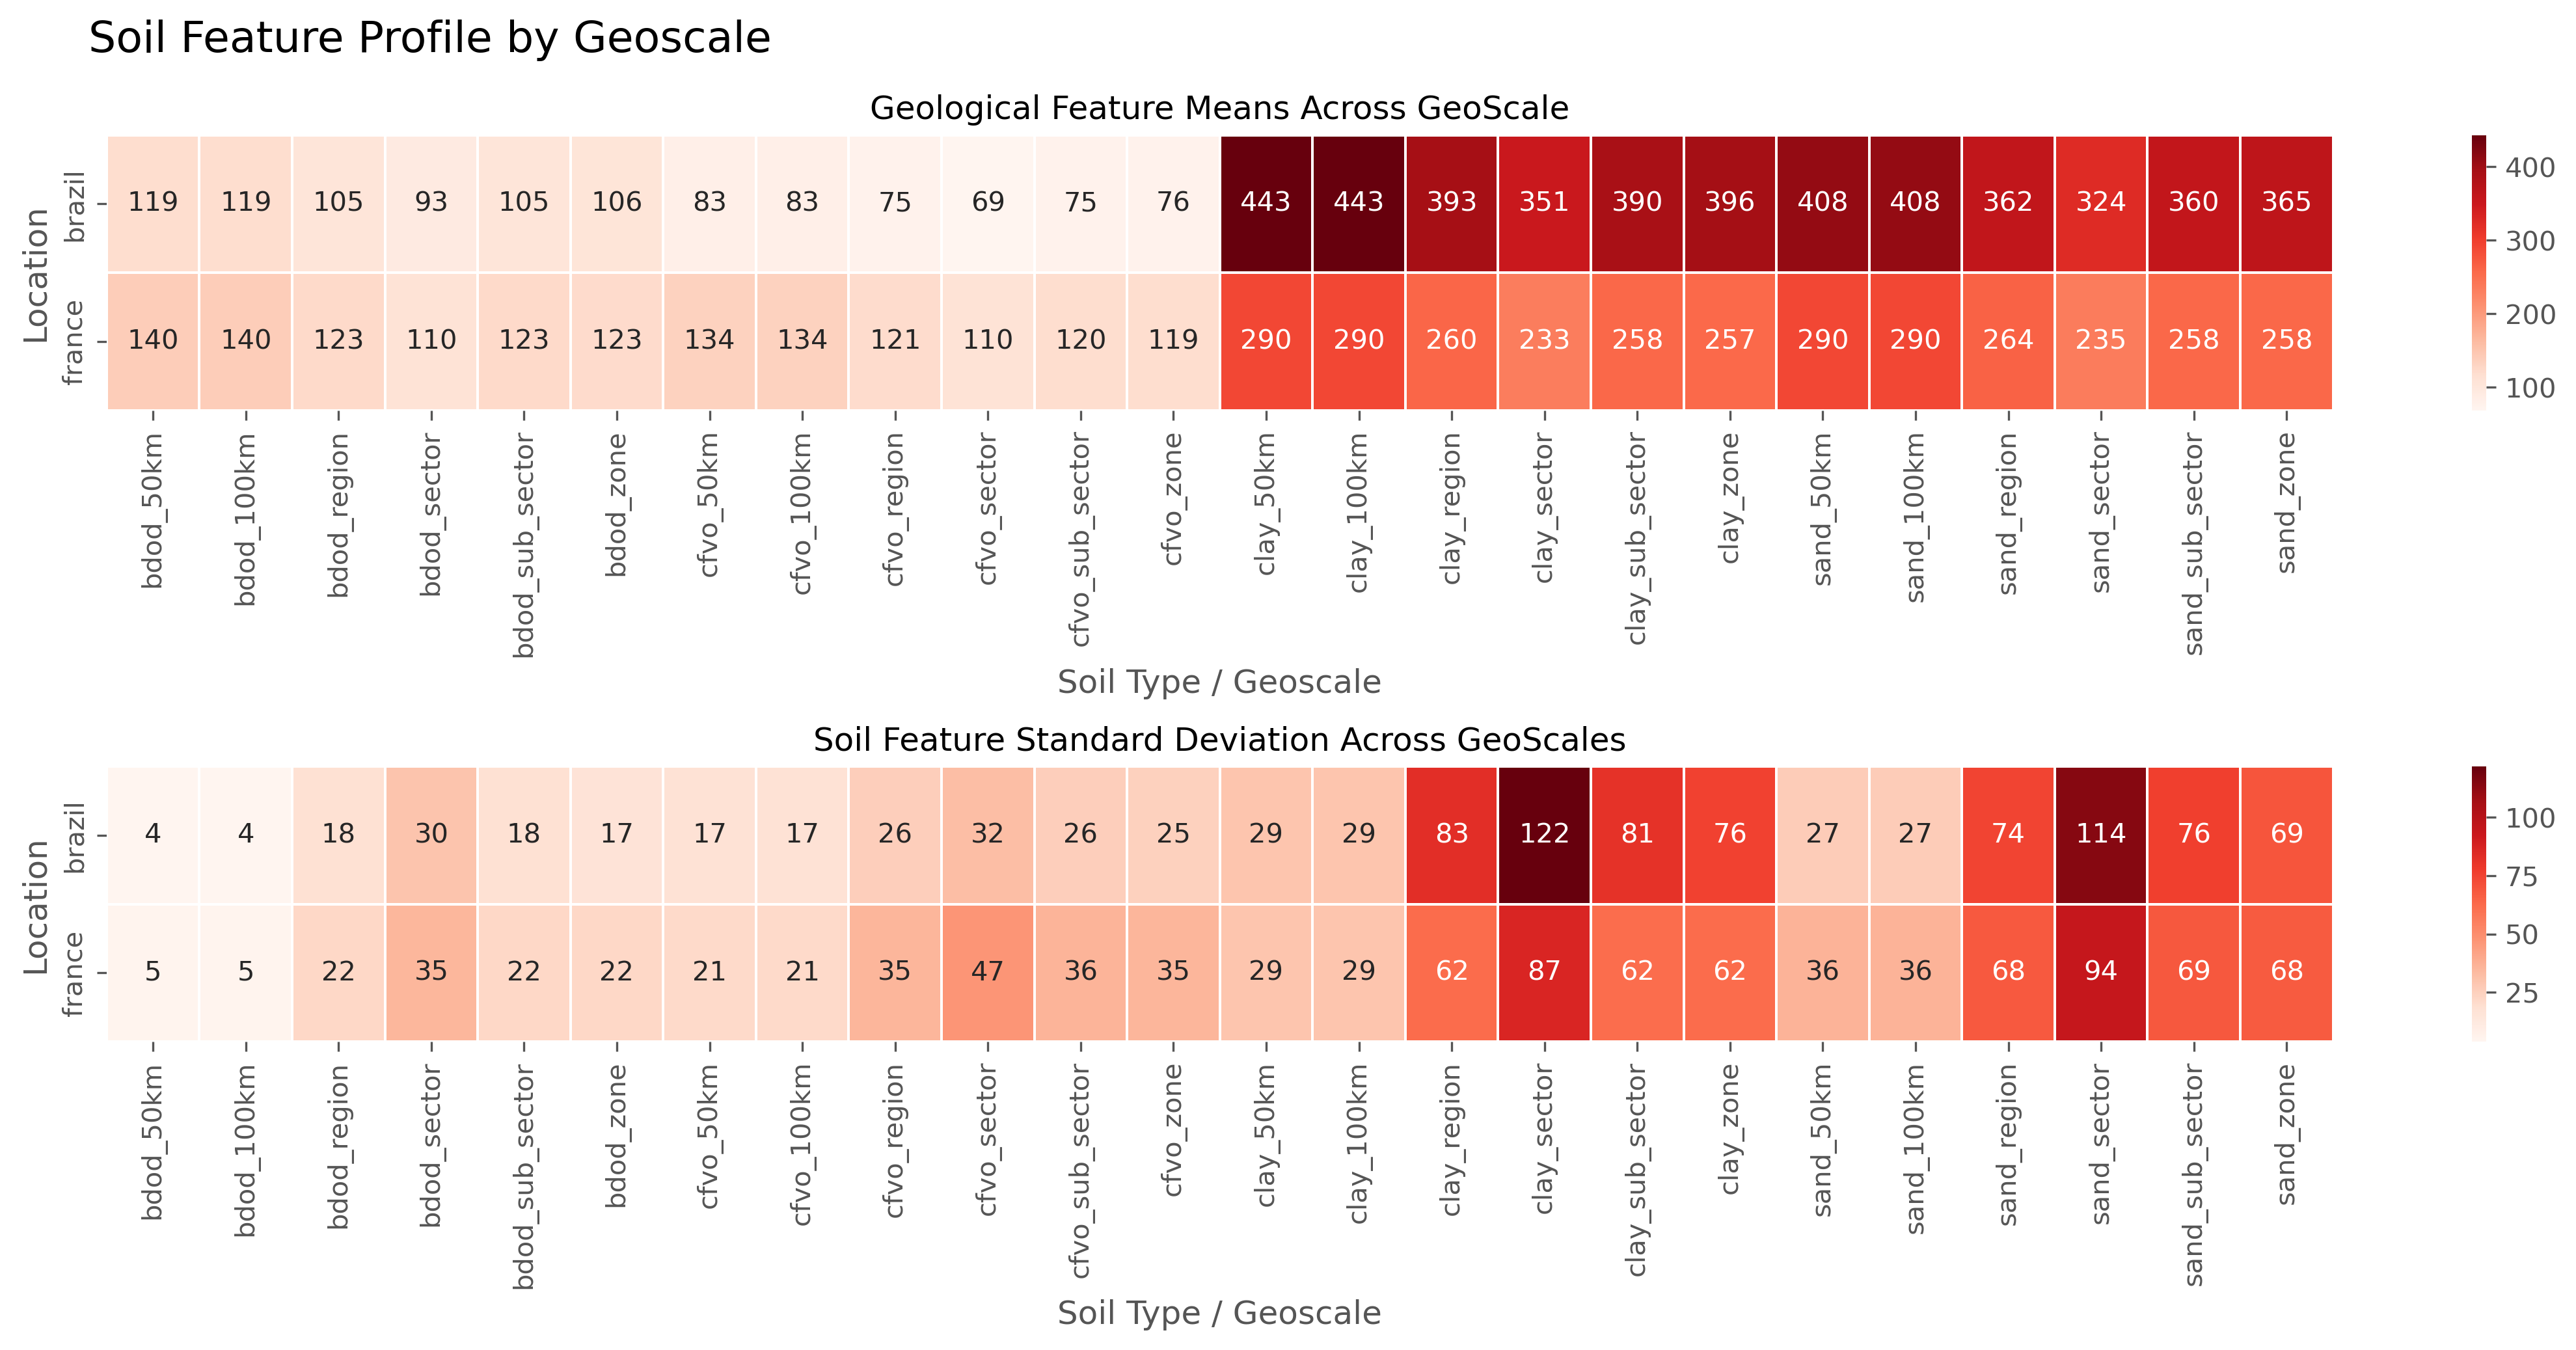
\includegraphics[width=\textwidth]{./assets/images/soil_feature_profile_geoscale.png}
            \caption{Soil Geoscales Profile}
            \label{fig:soil_feature_profile_geoscale}
        \end{subfigure}
        \caption{Top: Heatmap of soil feature means and standard deviations across depth per soil group. Bottom: Heatmap of soil feature means and standard deviations across geoscales per soil group. Fairly consistent means across depths and geoscales indicate minimal variaton in average soil characteristics. }
        \label{fig:soil_feature_profile}
    \end{figure}
    \vspace{3mm}

    \item{\textbf{Climate Features}}: 
    Climate data is aggregated at both the provided hydrological unit scale and within surrounding buffer zones to capture localized spatial variation. 
    Seasonal patterns are analyzed across locations, revealing consistent annual cycles across variables.
    \\ 
    Importantly, temperature(t2m) and evapotranspiration (evap) show opposing seasonal trends between northern and southern 
    hemisphere sites due to their geographic positions. To address this, we account for hemispheric differences by enforcing 
    location-specific constraints within the model, ensuring that the model interprets seasonal features within the appropriate 
    spatial context. This prevents confusion from features that exhibit similar meanings but opposite temporal behaviors across regions.
    \vspace{3mm}

    \item{\textbf{Rivers and Watersheds}}: Rivers are hierarchically ranked within each watershed, with lower values indicating 
    higher-order rivers. Brazil uses ranks 3–13, while France uses 1–7; we align these by subtracting 2 from Brazil’s ranks. 
    Rank 1 rivers in both countries show the highest average discharge. This calibrated river ranking offers a 
    valuable categorical spatial feature for modeling. Figure \ref{fig:river_ranking} shows river/station distribution and average discharge per river rank.\\
    \begin{figure}[h]
        \centering
        \begin{subfigure}[h]{1.0\textwidth}
            \centering
            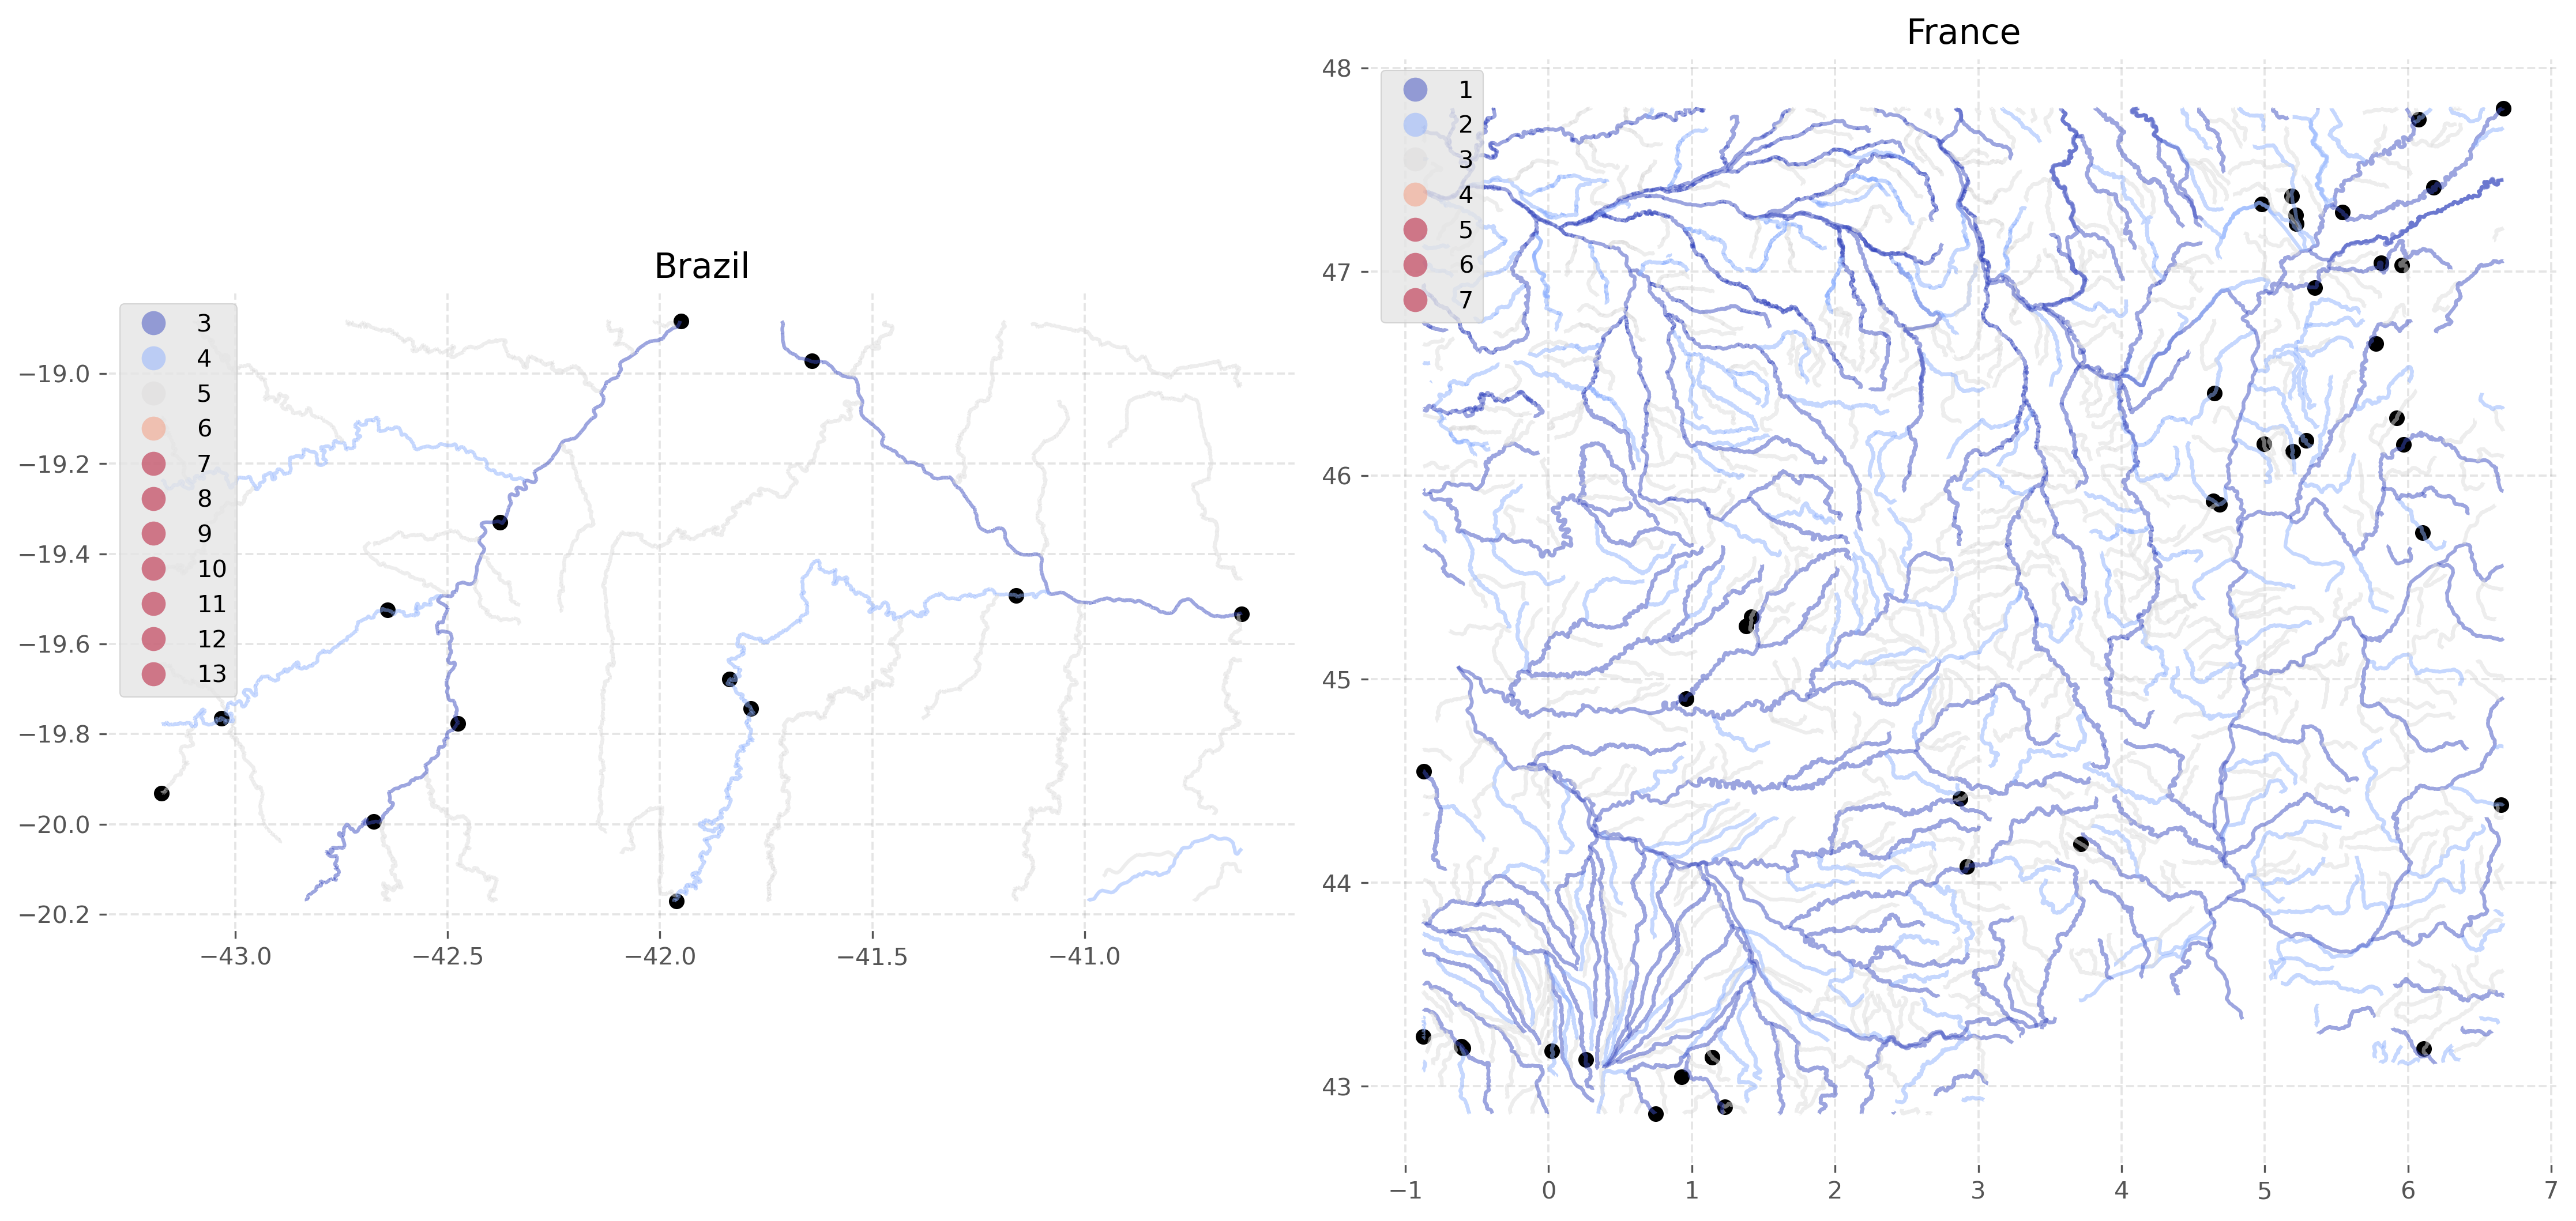
\includegraphics[width=\textwidth]{./assets/images/watershed_river_ranking.png}
            \caption{River / Stations Spatial Distribution}
            \label{fig:river_ranking_map}
        \end{subfigure}

        \begin{subfigure}[h]{1.0\textwidth}
            \centering
            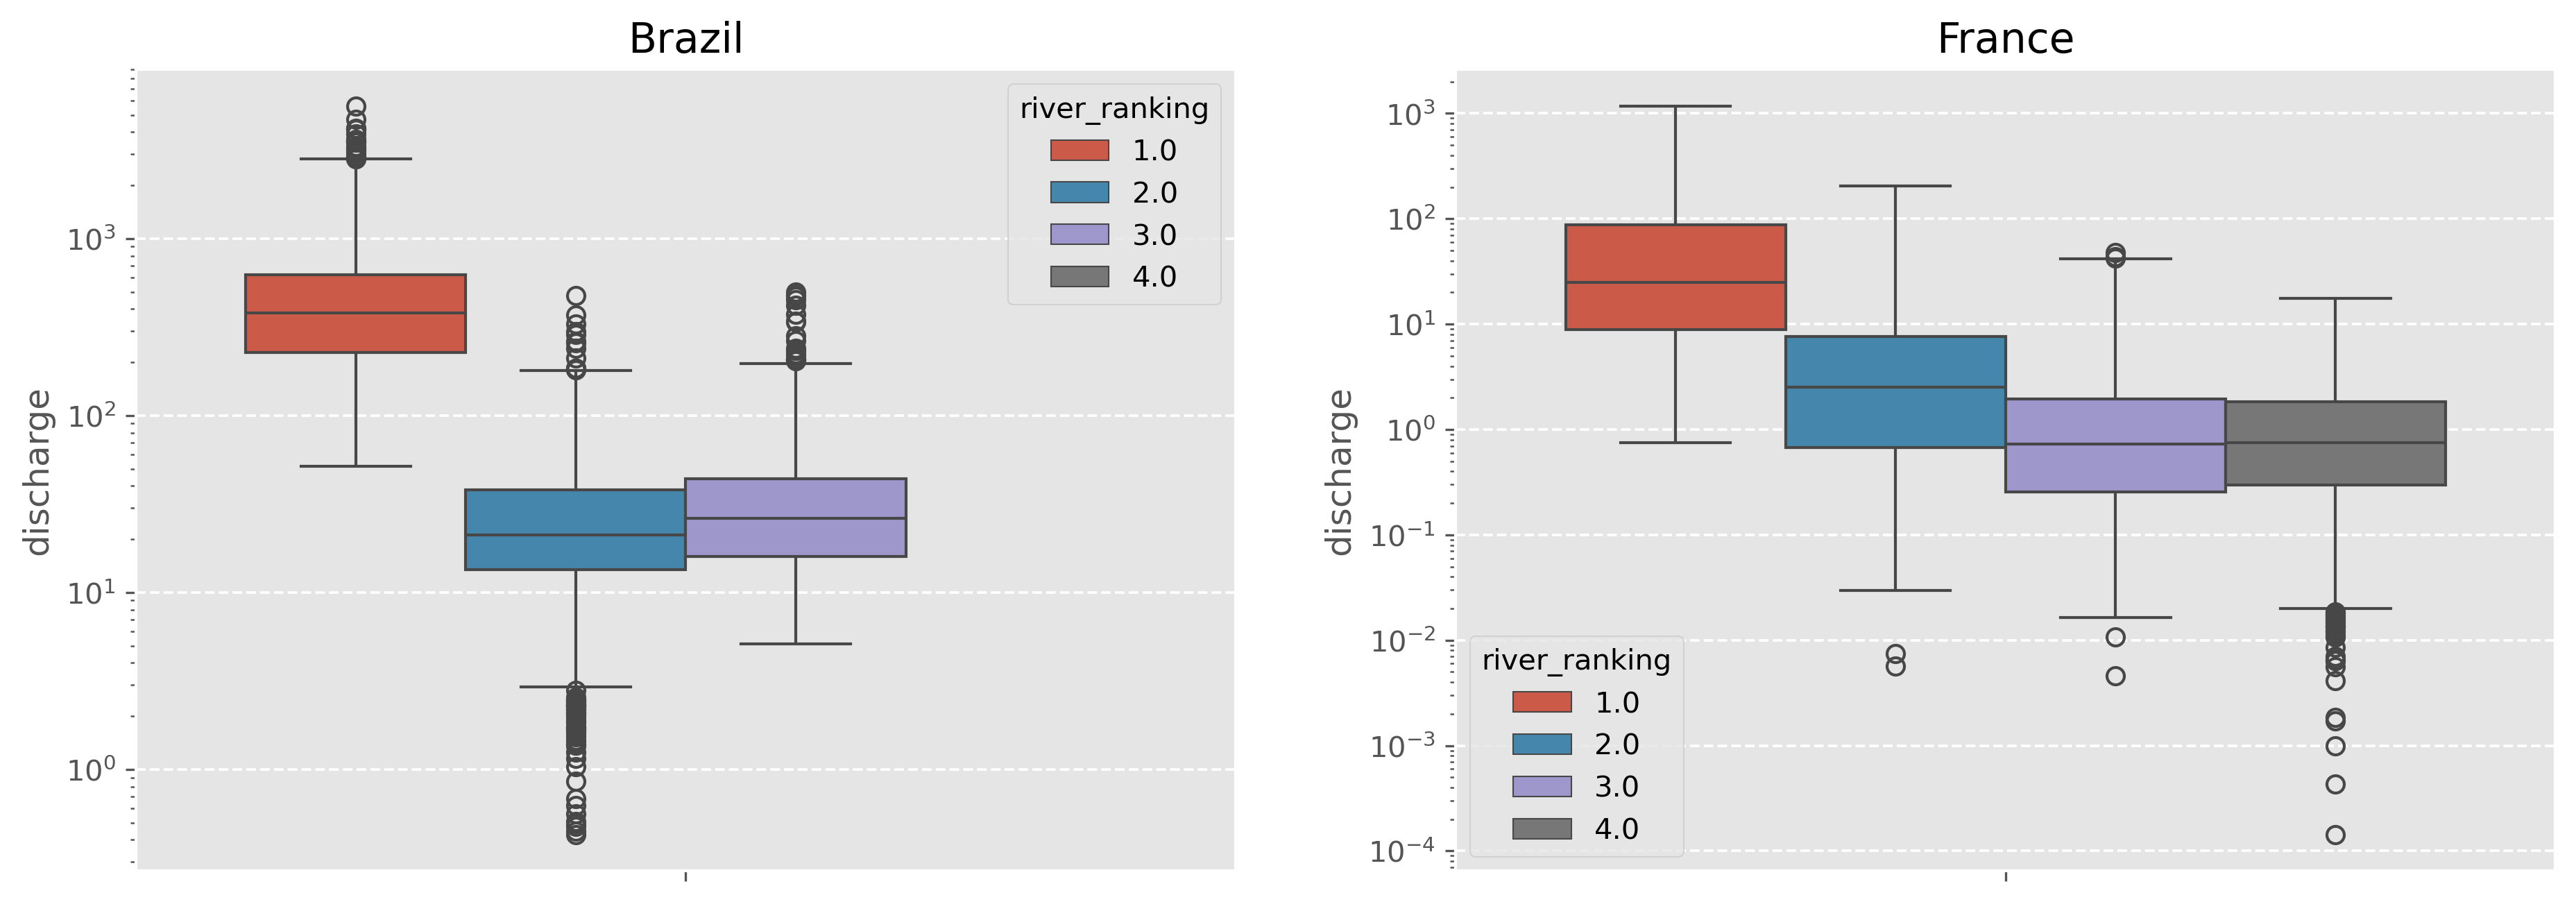
\includegraphics[width=\textwidth]{./assets/images/river_ranking_average_discharge.png}
            \caption{Average Discharge per River Rank}
            \label{fig:river_ranking_average_discharge}
        \end{subfigure}

        \caption{Top: Spatial distribution of top-ranked rivers in each location. Bottom: Average river discharge by rank, highlighting the dominance of higher-ranked rivers across countries}
        \label{fig:river_ranking}
    \end{figure}
    \vspace{3mm}

    \item{\textbf{Water Flow Patterns}}: Per-station analysis of water discharge reveals consistent flow patterns among stations located 
    along the same river systems. Across these stations, discharge exhibits strong annual seasonality with little to no long-term trend. 
    This behavior suggests empirical flow stationarity, indicating that historical discharge data remains representative of current 
    conditions. To leverage this, we compute the annual empirical flow, the historical mean discharge for each week of the year, and 
    include it as a model feature to capture expected seasonal behavior.\\ 
    \vspace{5mm}
    For stations not present in the training set, we estimate this feature by taking a weighted mean of the empirical flows from the 
    two geographically nearest stations. This approach provides a reasonable proxy, allowing the model to generalize seasonal discharge 
    patterns to ungauged locations.\\
    \vspace{3mm}

    \item{\textbf{Hydrographic Areas}}: High missingness at finer hydrographic scales (\textit{subsector and zone}) requires careful 
    imputation, which we address using proximity-based filling from neighboring hydro regions.

\end{itemize}

\subsubsection{Feature Engineering}
Feature engineering plays a vital role in enhancing model performance by creating informative and predictive variables \citep{kuhnjohnson2019}. 
Techniques such as lag features, seasonal decomposition, and trend extraction are widely recognized for their effectiveness in time series 
forecasting \citep{kuhnjohnson2019, hyndman2018}. In this work, we applied a range of techniques to capture spatial, temporal, and seasonal dynamics in the data
\begin{itemize}    
    \item \textbf{Lag Features:} Capture short-term dependencies (1, 2, 3, and 4 week lags)  of key variables (e.g., climate or flow). 1, 2, 3 and 4 weeks.
    
    \item \textbf{Rolling Features:} Include rolling statistics (mean and variance) over time windows to capture temporal variability.
    
    \item \textbf{Seasonal Features:} Encode week-of-year using Gaussian basis functions (4 or 8 components) to represent cyclical seasonal patterns.
    
    \item \textbf{Temporal Features:} Include calendar-based indicators such as day, week, and month.
    
    \item \textbf{Categorical Features:} Metadata such as region, land use, and sensor type encoded as categorical variables.
    
    \item \textbf{Out-of-Fold (OOF) Features:} To avoid data leakage, certain features were computed using out-of-fold strategies during cross-validation. This includes:
    \begin{itemize}
        \item \textit{Empirical Flow:} Historical flow statistics aggregated using only training fold data.
        \item \textit{KMeans Clustering:} Cluster assignments based on spatial or environmental patterns, generated per fold.
    \end{itemize}
\end{itemize}

\noindent\textbf{Total number of features after engineering:} \textit{[insert total here]}


\subsubsection{Feature Selection}
We perform feature selection to improve model robustness and reduce overfitting by identifying the most 
relevant predictors from different feature groups:
\begin{itemize}
    \item \textbf{Soil Features}: To reduce high dimensionality, we select a subset of informative and 
    non-redundant soil variables using statistical and model-based methods. This streamlines the 
    input space while retaining key spatial characteristics. We implement a two-step feature selection approach:
    \begin{enumerate}
        \item \textbf{Mutual Information Regression (MIR)  / Minimum Redundancy and Maximum Relevance (mRMR)}: We compute MIR scores in between each feature and the 
        target variable. MIR, used in mRMR feature selection frameworks, is well-suited for identifying relevant soil features due to its ability to capture both 
        linear and non-linear dependencies \citep{peng2005}, which are common in hydrological and environmental data. We retain 
        the top 10\% of features with the highest MIR scores, ensuring that the most informative predictors 
        are preserved.
        \vspace{5mm}
        \item \textbf{Correlation Filtering:} Within the MIR-selected subset, we apply correlation filtering to 
        remove redundant features. Feature pairs with a Pearson correlation coefficient greater than 0.9 are 
        identified, and the feature with the lower MIR score (or lesser domain relevance) is removed. This 
        reduces multicollinearity and improves model interpretability \citep{kuhnjohnson2019}.
    \end{enumerate}
    \item\textbf{Climate Features}: We prioritize causally relevant climate variables cross different spatial scales to promote model robustness 
    and generalizability. This ensures the model focuses on features with direct influence on hydrological responses. Similarly, we follow a 
    multi-step approach:
    \begin{enumerate}
        \item \textbf{Correlation Analysis:} We first analyze correlations at both local and global levels to identify 
        general patterns and dependencies within the climate data.
        \vspace{5mm}
        \item \textbf{Structured Causal Models:} To move beyond correlation and uncover causal effects, we apply structured causal models across spatial scales, 
        including local buffer zones and national regions. We estimate Average Treatment Effects (ATE) for key climate variables, quantifying their direct impact on the target 
        while adjusting for confounders. Directed Acyclic Graphs (DAGs) consistently identify temperature and precipitation as key drivers across regions, with soil water volume (SWVL) 
        emerging as a consistent driver in France. These findings are supported by counterfactual analyses that visualize potential outcomes under different climate conditions.
        \vspace{5mm}
        \item \textbf{Feature Importance:} Focusing on temperature, precipitation and soil moisture features, LightGBM is used to assess feature importance. Selecting the most predictive 
        features within these groups at different scales helps the model better represent key climate drivers.
    \end{enumerate}
\end{itemize}

\noindent This process yields a compact, non-redundant, and highly predictive feature set that captures both direct and complex interactions with the target variable.
\begin{figure}[!htp]
    \centering
    \begin{subfigure}[b]{0.48\textwidth}
        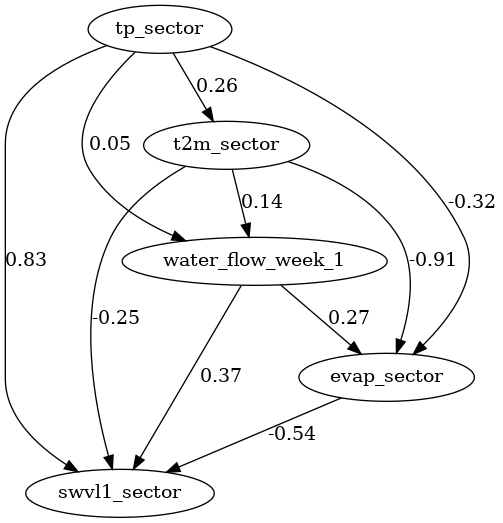
\includegraphics[width=\textwidth]{./assets/images/Brazil_sector_DAG.png}
        \caption{Sector-level DAG for Brazil}
        \label{fig:dag_brazil}
    \end{subfigure}
    \hfill
    \begin{subfigure}[b]{0.48\textwidth}
        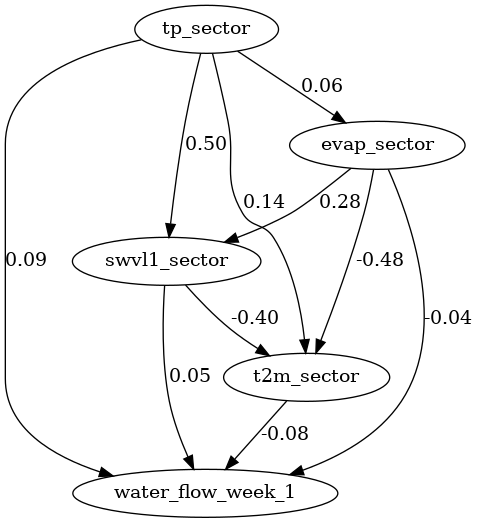
\includegraphics[width=\textwidth]{./assets/images/france_sector_DAG.png}
        \caption{Sector-level DAG for France}
        \label{fig:dag_france}
    \end{subfigure}
    \caption{Learned Directed Acyclic Graphs (DAGs) at the sector level, showing causal relationships between climate variables and the target in Brazil and France.}
    \label{fig:sector_dags}
\end{figure}

\begin{figure}[!htp]
    \centering
    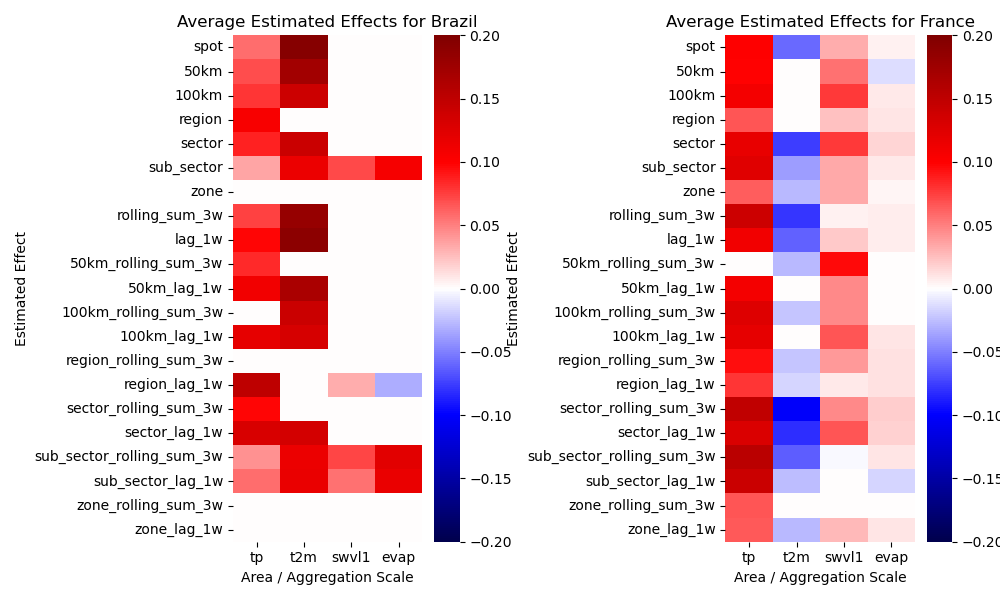
\includegraphics[width=0.85\textwidth]{./assets/images/ATEs.png}
    \caption{Estimated Average Treatment Effects (ATE) of key climate variables across spatial scales. Strong causal influence is observed from temperature and precipitation.}
    \label{fig:ate_heatmap}
\end{figure}

\subsubsection {Modelling FrameWork}
Gradient boosting methods have consistently demonstrated superior performance over other regression models in structured and environmental datasets \citep{shortridge2016, kumar2023}.
The core model is a Gradient Boosting Trees (GBT) regressor trained in a chained forecasting setup, where predictions from previous timesteps 
(e.g., \(\hat{y}_{t-1}, \hat{y}_{t-2}\)) are chained into input features for predicting future values \(\hat{y}_t\). 
This autoregressive structure enables multi-step forecasting while capturing temporal dependencies in the data.
\\ \\
To preserve temporal integrity, we use TimeSeriesSplit cross-validation. This ensures the model is always trained on past data and validated on future data. Each fold includes:
\begin{itemize}
    \item Computation of out-of-fold (OOF) and out-of-year (OOY) empirical flow statistics to avoid leakage.
    \item Fold specific KMeans clustering to group stations into hydrologically and geographically similar clusters.
    \item Fold-specific model training.
    \item Validation residuals computed and conformal calibration factors computed per cluster and per week
\end{itemize}

\noindent At test time, predictions are aggregated by computing:
\begin{itemize}
    \item The mean forecast.
    \item Quantiles (0.5, and 0.95) to characterize uncertainty.
    \item Qantile Conformal Calibration step is applied to improve the coverage and reliability of forecast intervals
\end{itemize}

\begin{figure}[htbp]
    \centering
    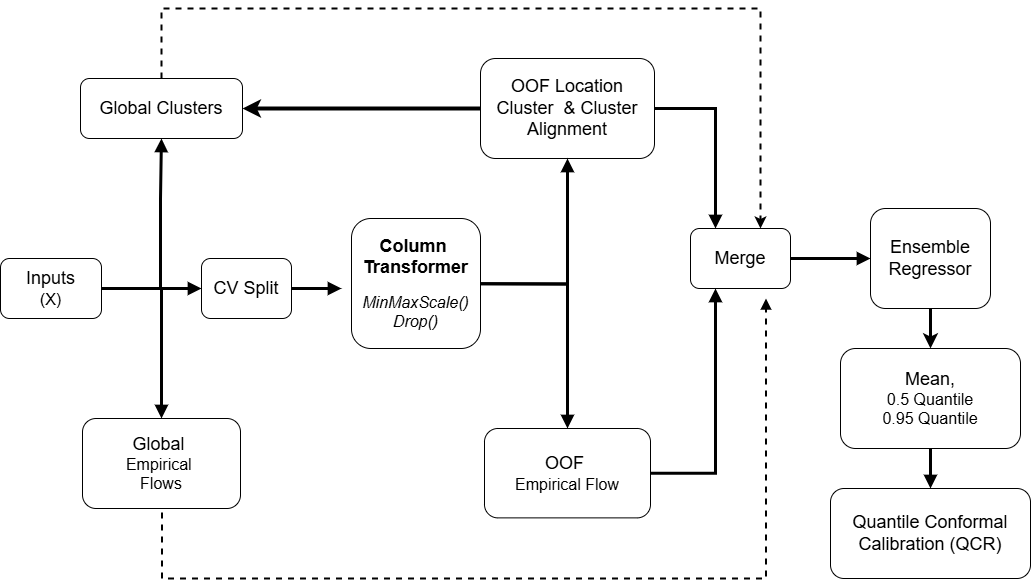
\includegraphics[width=1.0\textwidth]{./assets/model_2.png}
    \caption{Model Architecture}
    \label{fig:model_diagram}
\end{figure}

\begin{algorithm}[H]
\caption{Chained Ensemble Forecasting}
\begin{algorithmic}[1]
\State \textbf{Input:} Feature matrix $X$, target series $y$, number of folds $C$, number of ensemble models $n$, number of clusters $k$, conformal quantile level $\alpha$
\State \textbf{Output:} Forecasts with calibrated quantile intervals $\hat{y}$

\State Compute global KMeans clusters on $X_{\text{train}}$
\State Compute global empirical flow features per station $F$

\For{each fold $c = 1, \dots, C$}
    \State Split data into $X^{(k)}_{\text{train}}, X^{(k)}_{\text{val}}$ using ContiguousTimeSeriesSplit
    \State Compute KMeans clusters on $X^{(k)}_{\text{train}}$ (per-fold clustering)
    \State Align fold cluster IDs to global cluster ID
    \State Compute OOF and OOY empirical flow features (excluding fold/year)
    \State MinMax scaling of features to [0, 1]
    
    \For{each ensemble model $i = 1, \dots, n$}
        \State Train chained GBT regressor on $X^{(k)}_{\text{train}}$
        \State Predict on $X^{(k)}_{\text{val}}$ and store $\hat{y}^{(c,i)}$
    \EndFor
    
    \State Aggregate fold predictions: mean and quantiles
    \State Compute relative residuals $r^{(k)} = \frac{\hat{y}^{(k)} - y^{(k)}}{\hat{y}^{(k)} + \epsilon}$
    \State Compute $d{t} = Quantile_{1-\alpha}(r^{(k)})$ for each week $w$
    \State Store Conformal factors $d{t}$ for each cluster $c$ and week $w$
\EndFor
\State Preprocess test data $X_{\text{test}}$ using global clusters and empirical flow features
\State Predict on $X_{\text{test}}$ using the trained ensemble models
\State Compute mean and quantiles of predictions $\hat{y}_{\text{test}}$
\State Smooth conformal factors using weekly temporal blending.
\State Calibrate quantile intervals using smoothed conformal factors.
\State Return ensemble forecasts with calibrated intervals
\end{algorithmic}
\end{algorithm}

\subsubsection{Modelling Component Details}
\subsubsection*{ContiguousTimeSeriesSplit Cross Validation}
This validation strategy builds upon the \texttt{TimeSeriesSplit} approach from \textsc{scikit-learn}, where each fold's training set is a strict superset of the previous one, preserving the temporal ordering of the data. However, our method introduces two key modifications:

\begin{itemize}
    \item \textbf{Contiguous Validation:} Instead of using a fixed-size validation block for each fold, we validate on all remaining data after the training split. This allows the model to be assessed on the full available future horizon, improving robustness and generalization assessment.
    \vspace{5mm}
    \item \textbf{Minimum Training Size:} A constraint is imposed such that the first training fold must contain at least 50\% of the dataset. This ensures sufficient historical context is available for the initial training phase, preventing unstable model estimates due to data sparsity.
\end{itemize}

The fold structure for a 5-fold setup with years ranging from 1990 to 2004 is defined as follows:

\begin{table}[h!]

\centering
\begin{tabular}{ccc}
\hline
\textbf{Fold} & \textbf{Training Years} & \textbf{Validation Years} \\
\hline
1 & 1990--1998 & 1999--2004 \\
2 & 1990--1999 & 2000--2004 \\
3 & 1990--2000 & 2001--2004 \\
4 & 1990--2001 & 2002--2004 \\
5 & 1990--2002 & 2003--2004 \\
\hline
\end{tabular}
\caption{Contiguous expanding time series cross-validation structure.}
\end{table}

This approach ensures that:
\begin{itemize}
    \item Each model is trained only on past data relative to the validation set.
    \item The training window expands over time, simulating a real-world forecasting scenario.
    \item The evaluation is performed on all future data from the training endpoint, leading to more realistic performance metrics.
\end{itemize}

\subsubsection*{Data-Aware Global Clustering and Alignment }
To group stations into hydrologically similar regimes, we apply KMeans clustering on the full training data using a 
fixed number of clusters \( k \). This yields a global clustering structure that informs both model predictions and 
residual calibration.\\
To avoid data leakage in time series cross-validation, KMeans is recomputed independently within each training fold. 
Cluster centers vary between the global and fold-specific kMeans cluster ids, a well known label-switching issue in clustering. 
To ensure consistency of cluster assignments across cross-validation folds, we align fold-specific cluster ids with 
global cluster by solving an optimal assignment problem. Such alignment has been widely used in cluster ensembles and partition 
aggregation frameworks \citep{stephen2000, strehl2003}, with the optimization typically solved using the 
Hungarian algorithm \citep{kuhn1955}.\\

The alignment minimizes the total euclidean distance between fold-specific cluster centers 
\( C^{\text{fold}} \) and global cluster centers \( C^{\text{global}} \):

\begin{equation}
\min_{\pi \in \text{Perm}(k)} \sum_{i=1}^{k} \left\| C^{\text{fold}}_i - C^{\text{global}}_{\pi(i)} \right\|_2
\end{equation}

where \( \pi \) is a permutation of cluster indices. The aligned cluster IDs are then used to condition predictions and compute localized residual statistics.

\begin{algorithm}[!htp]
\caption{Data-Aware Global Clustering and Alignment}
\begin{algorithmic}[1]
\State \textbf{Input:} Training data \( X \), number of clusters \( k \), number of CV folds \( F \)
\State Fit global KMeans on \( X \) to obtain centers \( C^{\text{global}} \) and cluster IDs
\For{each fold \( f = 1 \) to \( F \)}
    \State Extract fold-specific training data \( X^{(f)} \)
    \State Fit KMeans on \( X^{(f)} \) to get centers \( C^{(f)} \)
    \State Compute cost matrix \( M_{ij} = \lVert C^{(f)}_i - C^{\text{global}}_j \rVert_2 \)
    \State Use Hungarian algorithm to solve:
    \[
        \min_{\pi \in \text{Perm}(k)} \sum_{i=1}^{k} M_{i,\pi(i)}
    \]
    \State Map fold-specific cluster IDs using optimal assignment \( \pi \)
    \State Assign aligned cluster labels to \( X^{(f)} \)
\EndFor
\State \textbf{Output:} Data with global-aligned cluster IDs for each fold
\end{algorithmic}
\end{algorithm}

\subsubsection*{Empirical Flow Features}
Empirical flow statistics are computed as the mean discharge per station and week, excluding the target year to prevent leakage. During training, global empirical flow is calculated and stored. After data splitting, empirical flow is recomputed using only the training fold data.

The inference function \texttt{\_get\_empirical\_prior} assigns empirical flow values for each data point as follows:

\begin{enumerate}
    \item If the station exists in the training priors, assign its empirical flow directly.
    \item Otherwise, estimate empirical flow by weighted averaging of the two nearest neighbor stations:
    \begin{itemize}
        \item Neighbors are selected based on river proximity, river ranking, and geographic location.
        \item Euclidean distances on latitude and longitude are computed to find the nearest neighbors.
        \item Weights are inverse-distance weighted to combine neighbors' empirical flows smoothly.
    \end{itemize}
\end{enumerate}

\noindent This method provides stable, leakage-free empirical priors for both seen and unseen stations during training and inference.

\bigskip

\begin{algorithm}[!htp]
\caption{Empirical Flow Feature Extraction}
\begin{algorithmic}[1]
\Require Dataframe $X$ with columns \texttt{week, year, station\_code}, empirical flow priors \texttt{priors}, station metadata \texttt{stations\_gdf}
\Ensure Dataframe $X$ augmented with empirical flow prior \texttt{empirical\_flow}

\State Assert columns \texttt{week, year, station\_code} exist in $X$
\State Copy $X$ to avoid modifying input
\ForAll{unique stations $s$ in $X$}
    \If{$s$ in columns of \texttt{priors}}
        \State Extract empirical flow data for station $s$
    \Else
        \State Find neighbors for $s$ by:
        \begin{itemize}
            \item Filtering stations with the same river and similar river ranking and location
            \item Calculating Euclidean distance based on latitude and longitude
            \item Selecting two nearest neighbors
        \end{itemize}
        \State Compute inverse distance weights for neighbors
        \State Compute weighted average of neighbors' empirical flow by week
    \EndIf
    \State Append station empirical flow data to results
\EndFor
\State Merge empirical flow results into $X$ by \texttt{station\_code} and \texttt{week}
\State \Return augmented $X$
\end{algorithmic}
\end{algorithm}

\subsubsection*{Relative Quantile Conformal Calibration} 
To address heteroscedasticity and the varying magnitudes of streamflow across regions and seasons, 
we propose \textbf{Relative Quantile Conformal Calibration (RQCC)} — an extension of conformal quantile 
calibration that adjusts prediction intervals using residuals scaled relative to the target value.
\\ \\ 
In standard quantile conformal prediction, coverage is achieved by computing residuals between predicted 
quantile bounds and observed values. For a model that outputs lower and upper quantile predictions 
$\hat{y}_t^{\text{lower}}$ and $\hat{y}_t^{\text{upper}}$, the standard conformal residual is:

\begin{equation}
r_t = \min\left( \hat{y}_t^{\text{upper}} - y_t,\; y_t - \hat{y}_t^{\text{lower}} \right)
\label{eq:absolute_residual}
\end{equation}

\noindent Using these residuals, the calibrated prediction interval is:

\begin{equation}
\left[ \hat{y}_t^{\text{lower}} - q_{1-\alpha},\; \hat{y}_t^{\text{upper}} + q_{1-\alpha} \right]
\label{eq:standard_interval}
\end{equation}
where $q_{1-\alpha}$ is the $(1 - \alpha)$-quantile of residuals from a held-out calibration set.
\\
\noindent However, in real-world hydrological applications, streamflow values can vary drastically 
between basins — from small ephemeral streams to major rivers. Applying absolute residuals in such 
cases results in mis-scaled intervals: overly wide in high-flow regimes and too narrow in low-flow areas. 
This undermines the interpretability and sharpness of calibrated intervals.
\\ \\ 
To normalize across such variation in target magnitudes, we define \textbf{relative residuals}:
\begin{equation}
r_t^{\text{rel}} = \frac{\min\left( \hat{y}_t^{\text{upper}} - y_t,\; y_t - \hat{y}_t^{\text{lower}} \right)}{y_t + \epsilon}
\label{eq:relative_residual}
\end{equation}
where $\epsilon > 0$ is a small constant (e.g., $10^{-6}$) added for numerical stability.
\\
Residuals are then grouped by \textbf{cluster} $c$ (e.g., hydrological regime) and \textbf{timestep} 
$t$ (e.g., season), and the conformal quantile is computed per group:
\begin{equation}
\delta_{c, t} = \text{Quantile}_{1 - \alpha} \left( \left\{ r_t^{\text{rel}} \right\}_{i \in \text{cluster } c} \right)
\label{eq:cluster_quantile}
\end{equation}

\noindent Finally, these relative quantile factors $\delta_{c, t}$ are used to expand the predicted interval proportionally:

\begin{equation}
\left[
\hat{y}_t^{\text{lower}} - \delta_{c, t} \cdot (y_t + \epsilon),\;
\hat{y}_t^{\text{upper}} + \delta_{c, t} \cdot (y_t + \epsilon)
\right]
\label{eq:relative_interval}
\end{equation}
\noindent This formulation maintains correct coverage while adapting to local flow characteristics, producing interpretable and consistent intervals across space and time.


\subsection{Experiments and Results}
\subsubsection{Experimental Setup}
We evaluate two variants of our model to assess the impact of soil features:
\begin{itemize}
    \item \textbf{Model A:} CatBoost model with the full feature set, including soil features.
    \item \textbf{Model B:} CatBoost model excluding all soil-related features.
\end{itemize}

Both models are trained using CatBoost with a quantile regression objective (quantile $\alpha=0.1$).
We employ a 5-fold contiguous cross-validation scheme with fold expansion. The splits are made by year to 
preserve temporal order and prevent data leakage. Model performance is evaluated using:
\begin{itemize}
    \item Negative Log-Likelihood (NLL)
    \item Interval Coverage (calibration of predicted quantiles)
\end{itemize}

\noindent This setup allows comparison of predictive accuracy, uncertainty quantification, and calibration 
between models with and without soil features.

\begin{table}[htbp]
\centering
\label{tab:metrics_comparison}
\begin{tabular}{lcccc}
\hline
\textbf{Model} & \textbf{OOF NLL} & \multicolumn{3}{c}{\textbf{Leaderboard Score}} \\
\cline{3-5}
 & & \textbf{Coverage} & \textbf{Temporal Split} & \textbf{SpatioTemporal Split} \\
\hline
A - \textit{With Soil Features} & \textbf{1.568} & \textbf{0.904} & \textbf{2.63} & 3.18 \\
B - \textit{Without Soil Features} & 1.572 & 0.900 & 2.65 & \textbf{3.05} \\
\end{tabular}
\caption{Performance Metrics Comparison of Models With and Without Soil Features}
\end{table}


\subsubsection{Explainability}
In this study, we focus on feature importance analyses aggregated across folds and weeks to interpret the model’s global behavior and temporal variation. While advanced explainability methods like SHAP values provide detailed local and global insights, they were not used here due to computational constraints and the complexity introduced by our ensemble model with multiple folds and repetitions.
\\
\noindent Instead, we rely on aggregated feature importance scores from the feature selection phase to capture variable influence on model predictions. Further explainability analyses, including residual diagnostics and local interpretability methods, remain valuable avenues for future work to enhance understanding of model performance and error characteristics.

\subsubsection*{Global Feature Importance}
Feature importances are computed using the average feature importances across all models in the ensemble.
\begin{figure}[ht]
\centering  
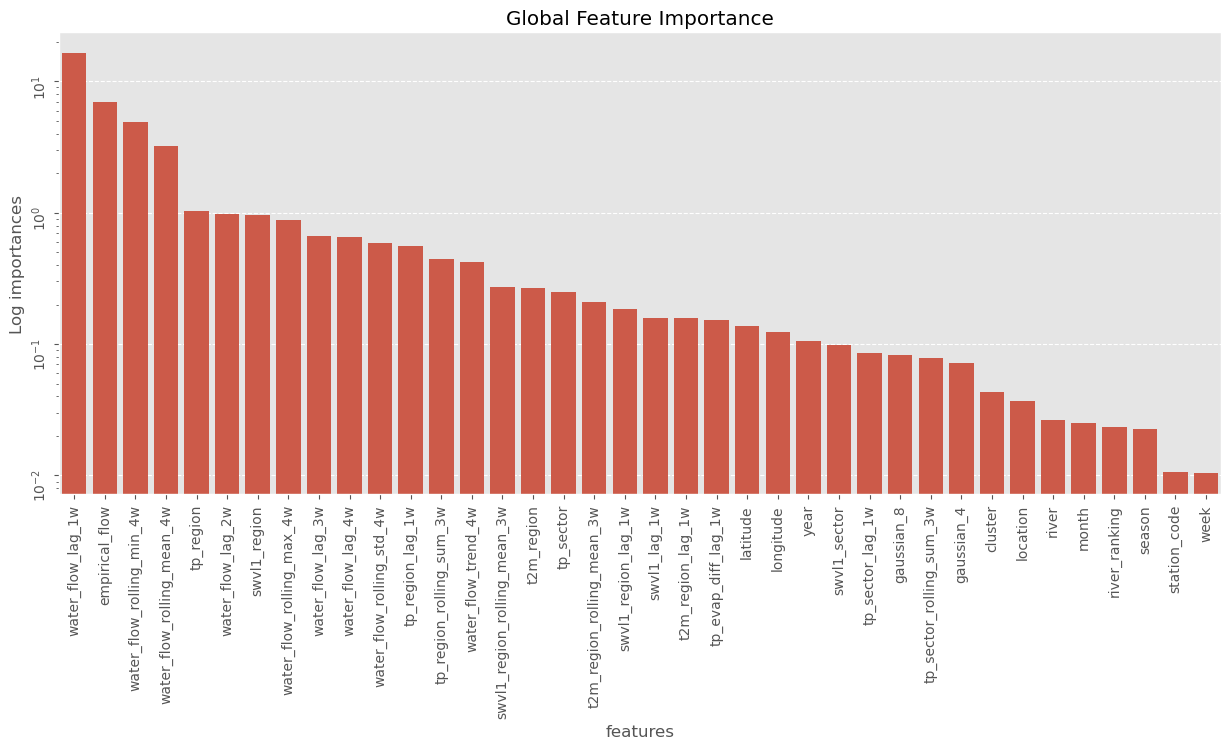
\includegraphics[width=1.0\textwidth]{./assets/images/global_feature_importance.png}
\caption{Global Feature Importance for the Model with Soil Features. The top 10 features are shown, with empirical flow and water flow lag features dominating the importance scores.}
\label{fig:global_feature_importance}
\end{figure}

\subsubsection*{Top Feature Importances per Fold and Week}
Feature importances are computed for each fold separately, allowing us to observe how feature relevance varies 
across different training and validation sets. The top 10 features per fold are summarized in Table 
\ref{tab:feat_importance_ranks_folds}, and Table \ref{tab:feat_importance_ranks_weeks} showing both their 
importance values and ranks within each fold and week respectively.
\begin{table}[!htp]
\centering
\small
\begin{tabular}{lccccc}
\hline
\textbf{Feature} & \textbf{Fold 1} & \textbf{Fold 2} & \textbf{Fold 3} & \textbf{Fold 4} & \textbf{Fold 5} \\
\hline
water\_flow\_lag\_1w           & 15.29 (1) & 16.73 (1) & 16.76 (1) & 16.51 (1) & 16.55 (1) \\
empirical\_flow               & 6.75 (2)  & 7.06 (2)  & 7.39 (2)  & 5.97 (2)  & 7.46 (2) \\
water\_flow\_rolling\_min\_4w & 6.12 (3)  & 4.98 (3)  & 5.44 (3)  & 4.18 (4)  & 3.85 (3) \\
water\_flow\_rolling\_mean\_4w & 3.66 (4)  & 3.36 (4)  & 2.78 (5)  & 3.70 (3)  & 2.56 (4) \\
tp\_region                   & 1.02 (7)  & 1.03 (5)  & 0.96 (6)  & 1.08 (6)  & 1.06 (6) \\
swvl1\_region                & 0.90 (8)  & 0.99 (6)  & 0.92 (7)  & 1.17 (5)  & 0.80 (7) \\
water\_flow\_lag\_2w           & 1.12 (6)  & 0.86 (9)  & 0.92 (8)  & 0.88 (7)  & 1.15 (5) \\
water\_flow\_lag\_3w           & 0.75 (9)  & 0.88 (7)  & 0.71 (10) & 0.77 (8)  & 0.50 (9) \\
water\_flow\_lag\_4w           & 0.64 (10) & 0.64 (10) & 0.75 (9)  & 0.77 (9)  & 0.62 (8) \\
water\_flow\_rolling\_max\_4w & 1.62 (5)  & 0.64 (11) & 1.02 (5)  & 0.72 (10) & -         \\
water\_flow\_rolling\_std\_4w & -         & 0.86 (8)  & -         & 0.68 (11) & -         \\
tp\_region\_lag\_1w           & -         & -         & -         & -         & 0.50 (10) \\
\hline
\end{tabular}
\caption{Top feature importances (values) and ranks (in parentheses) per fold. "-" indicate feature not in top 10 for corresponding fold.}
\label{tab:feat_importance_ranks_folds}
\end{table}

\begin{table}[!htp]
\centering
\begin{tabular}{lcccc}
\hline
\textbf{Feature} & \textbf{Week 1} & \textbf{Week 2} & \textbf{Week 3} & \textbf{Week 4} \\ 
\hline
water\_flow\_lag\_1w & 15.84 (1) & 17.22 (1) & 17.05 (1) & 15.35 (1) \\
empirical\_flow & 6.91 (2) & 7.02 (2) & 6.32 (2) & 7.45 (2) \\
water\_flow\_rolling\_min\_4w & 5.86 (3) & 5.34 (3) & 4.21 (3) & 4.24 (3) \\
water\_flow\_rolling\_mean\_4w & 3.57 (4) & 3.17 (4) & 3.28 (4) & 2.83 (4) \\
tp\_region & 1.05 (7) & 0.96 (5) & 1.02 (6) & 1.1 (5) \\
swvl1\_region & 0.95 (8) & 0.93 (6) & 1.13 (5) & 0.81 (7) \\
water\_flow\_rolling\_max\_4w & 1.34 (5) & 0.91 (7) & 0.81 (8) & - \\
water\_flow\_lag\_2w & 1.11 (6) & 0.88 (8) & 0.9 (7) & 1.05 (6) \\
water\_flow\_lag\_4w & - & - & 0.81 (9) & 0.6 (8) \\
tp\_region\_rolling\_sum\_3w & - & - & - & 0.52 (9) \\
water\_flow\_rolling\_std\_4w & 0.93 (9) & - & - & 0.52 (10) \\
water\_flow\_lag\_3w & 0.82 (10) & 0.71 (9) & 0.65 (10) & - \\
tp\_region\_lag\_1w & - & 0.62 (10) & - & - \\
\hline
\end{tabular}
\caption{Top feature importances (values) and ranks (in parentheses) per week. "-" indicates feature not in top 10 for corresponding week.}
\label{tab:feat_importance_ranks_weeks}   
\end{table}
\noindent The tables show that water flow lag features consistently rank among the top predictors across folds and weeks, indicating their strong temporal influence on streamflow. Empirical flow also remains a key feature, reflecting its importance as a hydrological prior. Other features such as rolling statistics and regional climate variables vary in importance depending on the fold or week, suggesting that local hydrological conditions and seasonal patterns significantly affect model predictions.

\subsubsection{Robustness}
\label{sec:robustness}

Given the model's complexity and reliance on diverse features, we assess robustness across three dimensions: out-of-fold consistency, spatiotemporal generalization, and interval reliability.

\subsubsection*{Out-of-Fold Validation}
We evaluate the model's performance across five validation folds to ensure stable behavior across different training splits. Table~\ref{tab:mae_per_fold_week} reports the Mean Absolute Error (MAE) for each week.

\begin{table}[ht]
\centering
\begin{tabular}{lcccc}
\hline
\textbf{Fold} & \textbf{Week 1} & \textbf{Week 2} & \textbf{Week 3} & \textbf{Week 4} \\
\hline
fold\_1 & 14.300 & 17.446 & 24.149 & 27.747 \\
fold\_2 & 14.387 & 17.384 & 24.414 & 27.469 \\
fold\_3 & 14.008 & 17.205 & 24.654 & 27.470 \\
fold\_4 & 14.125 & 17.065 & 25.264 & 28.311 \\
fold\_5 & 12.005 & 16.657 & 23.105 & 22.378 \\
\hline
\end{tabular}
\caption{Mean Absolute Error (MAE) per fold and week on the out-of-fold validation set.}
\label{tab:mae_per_fold_week}
\end{table}

\noindent The model maintains consistent performance across folds, with lower errors in later folds—likely due to more historical data becoming available (see Table~\ref{tab:mae_per_fold_week}). Errors increase with forecasting horizon, reflecting compounding uncertainty and growing temporal distance from observed lags.

\subsubsection*{Spatiotemporal Generalization}
To evaluate the model's ability to generalize across spatial and temporal domains, we introduce a held-out spatiotemporal validation split. This includes four stations from France and two from Brazil, excluded entirely from training. Table~\ref{tab:spatiotemporal_generalization_aggregated} shows MAE across weeks on this combined set.

\begin{table}[ht]
\centering
\begin{tabular}{lcccc}
\hline
\textbf{Fold} & \textbf{Week 1} & \textbf{Week 2} & \textbf{Week 3} & \textbf{Week 4} \\
\hline
fold\_1 & 14.677 & 18.508 & 26.391 & 29.732 \\
fold\_2 & 14.584 & 18.778 & 26.164 & 30.165 \\
fold\_3 & 14.893 & 18.533 & 26.309 & 29.712 \\
fold\_4 & 15.025 & 19.117 & 27.309 & 30.653 \\
fold\_5 & 13.129 & 17.930 & 24.705 & 23.950 \\
\hline
\end{tabular}
\caption{Aggregated spatiotemporal generalization performance on held-out stations and temporal split.}
\label{tab:spatiotemporal_generalization_aggregated}
\end{table}

\noindent As shown in Table~\ref{tab:spatiotemporal_generalization_aggregated}, performance degrades slightly on the spatiotemporal set, though it remains within acceptable bounds. To provide fairer comparisons across stations, we report station-normalized MAE in Table~\ref{tab:spatiotemporal_generalization}.

\begin{table}[ht]
\centering
\begin{tabular}{lcccc}
\hline
\textbf{Split} & \textbf{Week 1} & \textbf{Week 2} & \textbf{Week 3} & \textbf{Week 4} \\
\hline
Temporal\_split & \textbf{0.287} & \textbf{0.464} & 0.569 & \textbf{0.605} \\
Spatio\_temporal\_split & 0.348 & 0.485 & \textbf{0.564} & \textbf{0.605} \\
\hline
\end{tabular}
\caption{Station-normalized MAE across weeks for temporal and spatiotemporal splits.}
\label{tab:spatiotemporal_generalization}
\end{table}

\noindent The normalized MAE in Table~\ref{tab:spatiotemporal_generalization} shows slightly better results on the temporal split, but the gap is narrow—highlighting the model’s generalization ability even on unseen spatial regions.

\subsubsection*{Prediction Interval Width}

We also assess uncertainty calibration via the prediction interval width, normalized per station. Results are presented in Table~\ref{tab:normalized_interval_width}.

\begin{table}[ht]
\centering
\begin{tabular}{lcccc}
\hline
\textbf{Split} & \textbf{Week 1} & \textbf{Week 2} & \textbf{Week 3} & \textbf{Week 4} \\
\hline
Temporal\_split & 1.178 & 1.671 & 1.889 & 1.969 \\
Spatio\_temporal\_split & 1.188 & 1.651 & 1.746 & 1.763 \\
\hline
\end{tabular}
\caption{Station-normalized prediction interval width across weeks for temporal and spatiotemporal splits.}
\label{tab:normalized_interval_width}
\end{table}

\noindent As shown in Table~\ref{tab:normalized_interval_width}, prediction intervals are slightly tighter for spatiotemporal splits, which may lead to undercoverage and elevated NLL scores. This suggests that while the model is confident, it may be underestimating uncertainty on unseen stations.

\subsubsection*{Discussion on Generalization and Uncertainty}

The observed gap between out-of-fold and leaderboard scores highlights key opportunities for improvement. Strong out-of-fold performance (Table~\ref{tab:mae_per_fold_week}) provides a solid foundation, while the results on unseen stations (Tables~\ref{tab:spatiotemporal_generalization}, \ref{tab:normalized_interval_width}) emphasize areas for better spatial generalization and uncertainty calibration.

Enhancements such as stronger regularization, increased training diversity, and refined spatiotemporal validation can help bridge this gap. Overall, the model demonstrates strong robustness with promising potential for deployment across varied hydrological settings.


\subsubsection{Frugality Analysis}
\label{sec:frugality}
The final model is an ensemble composed of 15 base chained regression learners per fold, trained across $K$ cross-validation splits, resulting in a total of $15 \times K \times 4$  models. This structure enhances predictive performance and stability but introduces additional computational and memory overhead.

\subsubsection*{Data Usage and Efficiency}
The model uses moderate-sized datasets with internally generated features such as out-of-fold (OOF) predictions and empirical flow estimates. While scalable, the generation of OOF features adds to the overall training complexity. No external datasets are required beyond the primary climate and site-level inputs.

\subsubsection*{Training Runtime and Inference Efficiency}
Training time increases with the number of base learners but can be parallelized across folds and ensemble members. Reducing the folds and/or number of models per fold substantially decreases latency and memory usage, making the model more deployable in resource-constrained environments.

\begin{table}[H]
\centering
\caption{Model Configuration Trade-offs}
\begin{tabular}{lccccc}
\hline
\textbf{Configuration} & \textbf{OOF NLL} & \textbf{Models} & \textbf{Train (m)} & \textbf{Inference (ms)} & \textbf{Size (MB)} \\
\hline
Full Ensemble (15/fold) & 1.57 & 300 & ~20 & 2820 & $\sim$78 \\
Reduced Ensemble (10/fold) & 1.58 & 200 & ~14 & 2260 & $\sim$58.4 \\
Single Fold (15) & 1.588 & 60 & ~8 & - & $\sim$27.18 \\

\hline
\end{tabular}
\label{tab:frugality}
\end{table}

\section{Part 2 - Policy Design and Optimizattion}
The second phase of the competition focused on the design and optimization of policies to govern the 
allocation of shared water resources in a game theory simulation environment.
\\ \\
Effective water policy must balance ecological protection, equitable access, and economic stability, reflecting 
the broader principles of sustainable water management that call for joint consideration of social, economic and environmental 
needs \citep{wang2025}. 
Our approach emphasizes fairness—allocating water by priority—while ensuring sustainability for downstream ecosystems and resilience 
under uncertainty.We iteratively test the simulation environment, manually adjusting key parameters (e.g., demand and penalty multipliers) 
to understand how policy rules affect economic and ecological outcomes. This process aligns with simulation-based optimization approaches in 
water resource research, which are often used to explore policy trade-offs under uncertainty \citep{tian2019,tang2021,fu2020}. 
\\ \\
We observed the incentive function shapes drive cooperation and economic stability, while quota allocations and actor priorities impact ecological health.
Based on these insights, we design adaptive policies that respond to environmental signals, guiding agents toward 
sustainable behavior. Our framework includes:
\begin{itemize}
    \item Simulation Environment Parallelization
    \item Quota Function: A priority-aware allocation mechanism with configurable thresholds.
    \item Incentive Function: A fine/subsidy structure with both stepwise and smooth variants.
    \item Multiobjective Optimization : A Pareto-front approach using Optuna to discover trade-offs between economic efficiency and ecological viability.
    \item Policy Regulator Framework: A python class that encapsulates the policy design and optimization process to yield simulation-ready policy functions.  
\end{itemize}
\noindent This framework allows us to explore how adaptive, minimalistic rules can guide cooperation and robustness in a complex, uncertain environment.
\subsection{Simulation Environment Parallelization}
At the heart of the policy evaluation workflow is the $multi\_scenario\_analysis$ function, responsible 
for executing simulations across a range of behavioral and environmental configurations. This function 
plays a central role in assessing the robustness and generalizability of policy designs, ensuring that 
any proposed strategy is evaluated across diverse and uncertain scenarios. 
\\ \\
The original function is effective in exploring these scenarios sequentially. The parallelization of the 
$multi\_scenario\_analysis$ function is a crucial step in optimizing the policy evaluation process. 
By leveraging Python's concurrency capabilities, we can execute multiple scenarios simultaneously, 
significantly reducing the time required for each evaluation cycle. This is particularly important in the 
context of policy optimization, where rapid feedback on policy performance is essential for iterative 
refinement and decision-making.
\\ \\
We also enhance the function's flexibility to allow specifying custom scenario subsets—enabling 
targeted evaluation and more efficient use of compute resources during optimization. These enhancements 
integrate seamlessly with optuna’s multi-objective optimization framework, allowing for large-scale policy search.
\\ \\
Together, these improvements reduce the runtime of a 700 turns, 10 iterations simulation from approximately 
3 hours to less than 20 minutes per full evaluation cycle.

\subsection{Quota Function Design}
In water-stressed systems, resource allocation must carefully balance fairness, actor resilience, and 
ecological resilience — ensuring that critical needs are met without compromising the long-term health 
of the environment. This becomes especially important during crisis conditions, where water scarcity 
intensifies and allocation decisions carry systemic consequences.
\\ \\
\noindent To address this challenge, we propose a quota policy function for allocating water across multiple actors 
with varying demands and priorities. 

\subsection{Policy Mechanism}
The function is guided by three key parameters:

\begin{itemize}
    \item \textbf{rate ($r$)}: The baseline proportion of each actor's demand that is fulfilled during non-crisis periods. 
    This controls total water use and supports ecosustainability by preventing excessive extraction even under normal conditions.
    \item \textbf{priority\_effect ($p_e$)}: A tuning parameter that controls how much high-priority actors are favored during crises.
    When priority effect is 0, non-low-priority actors share water equally (relative to demand). Higher values increasingly concentrate 
    allocation toward the highest-priority actors. Low-priority actors receive no water during alert and crises, based on prior analysis 
    showing they maintain high buffer-to-demand ratios and can self-sustain through temporary shortages.
    \item \textbf{crisis\_rate ($r_c$)}: The overall reduction in water availability during crisis or alert conditions, defining what 
    percentage of each actor’s demand (before applying priority) is considered for allocation. This simulates external constraints and enforces 
    ecosustainability by capping water use according to environmental thresholds.
\end{itemize}  
\subsection{Mathematical Formulation}
Let:
\begin{itemize}
  \item $\mathbf{D} = (D_1, D_2, \dots, D_n)$: vector of average water pumped per actor.
  \item $\mathbf{P} = (P_1, P_2, \dots, P_n)$: vector of actor priorities.
  \item $\text{crisis\_level}(c) \in \mathbb{R}$: severity of crisis (non-crisis if $\leq -1$).
  \item $\mathrm{scale}(s) = \left( \mathrm{MAD\_score}(\mathbf{D}) \right)^{-0.25}$: Mean Absolute Deviation of avg\_pump to identify high demand actors.
  \item $ r \in [1, \infty)$
  \item $r_c \in [0, \infty)$
  \item $p_e \geq 0$
  \item $\mathbb{I}_{\{P_i > 0\}}$: indicator function (1 if $P_i > 0$, else 0)
\end{itemize}

\textbf{Quota per actor} $q_i$ is defined as:

\[
q_i =
\begin{cases}
D_i \cdot r, & \text{if } \text{crisis\_level} \leq -1 \\[12pt]
\displaystyle
\frac{A_i}
{\sum\limits_{j=1}^n A_j}
\cdot W, & \text{otherwise}

\end{cases}
\]
where allocation weights $A$ during crisis is
\[
A = D_i \cdot \exp\left(P_i \cdot c \cdot p_e \cdot s \right) \cdot \mathbb{I}_{\{P_i > 0\}}
\]
and the total available water $W$ during crisis is:
\[
W = \frac{r_c}{\max(1, c)} \cdot \sum_{k=1}^n D_k \cdot \mathbb{I}_{\{P_k > 0\}}
\]

\section{Incentives Policy Design}
This incentives policy promotes \textbf{equitable and sustainable water use} by influencing actor behavior 
through \textbf{penalties for overuse} and \textbf{rewards for conservation}. It is designed to balance three core objectives:

\begin{itemize}
    \item \textbf{Fairness:} Incentives are scaled relative to each actor’s quota and demand, ensuring proportionate responses.
    \item \textbf{Equity:} The policy accounts for actor priority, offering more leniency to high-priority users while maintaining system-wide consistency.
    \item \textbf{Ecosustainability:} Incentive strength increases with crisis severity, encouraging conservation and system resilience under stress.
\end{itemize}

\subsubsection{Policy Mechanism}
\subsubsection*{Core Mechanism}
The policy calculates an \textit{incentive rate} based on the difference between actual water use and the actor’s quota 
(the \textit{overuse}). This rate is scaled by:

\begin{itemize}
    \item \textbf{policy\_rate ($r_p$):} Governs the overall intensity of incentives, controlling how strongly behavior 
    is encouraged or discouraged.
    \item \textbf{equity\_spread ($eqs$):} Adjusts the baseline leniency by influencing how much the actor’s priority 
    affects the scaling of incentives. A higher equity spread means more leniency towards higher-priority actors.
    \item \textbf{crisis\_sensitivity ($cs)$:} Dictates how sharply the incentive system reacts to crisis severity. 
    When crisis levels increase, incentives become more severe, compelling actors to reduce consumption.
\end{itemize}

\subsubsection*{Subsidy and Fine Asymmetry}
The incentive function is \textbf{asymmetric} between penalties and subsidies:

\begin{itemize}
    \item The \textbf{subsidy\_fine\_ratio ($\gamma$)} controls the relative steepness of rewards (subsidies) versus penalties 
    (fines). This allows the policy to fine-tune whether conservation is rewarded more gently or harshly compared to overuse penalties.
    \item Both penalties and subsidies are bounded by maximum caps - \textbf{max\_fine\_weight ($F_{max}$)} and 
    \textbf{max\_subvention\_weight ($S_{max}$)}. This prevents excessively harsh fines or unreasonably large subsidies.
\end{itemize}

\subsubsection*{Crisis Memory and Dynamic Prioritization}
An additional important feature is the policy’s ability to \textbf{incorporate historical crisis information} to 
modulate responses dynamically:

\begin{itemize}
    \item The policy tracks whether a \textit{crisis is ongoing}, based on both current water availability and 
    consumption patterns.
    \item A parameter \(\alpha\) balances how much weight to give to \textit{past crisis conditions} versus the 
    \textit{current crisis status}.
    \item This memory effect allows the system to \textbf{anticipate future water shortages} and 
    \textbf{adjust crisis severity accordingly}. As a result, if the crisis persists over multiple iterations, the crisis level can escalate, increasing 
    the strictness of incentives.

\end{itemize}

\subsubsection{Mathematical Formulation}
Let:
\begin{itemize}
    \item $\mathbf{D} = (D_1, D_2, \dots, D_n)$: vector of average water pumped per actor.
    \item $\mathbf{P} = (P_1, P_2, \dots, P_n)$: vector of actor priorities.
    \item $\mathbf{C} \in \mathbb{R}$: vector of severity of crisis (non-crisis if $\leq -1$).
    \item $\mathbf{A} = (A_1, A_2, \dots, A_n)$: vector of water pumped by each actor.
    \item $\mathbf{W} = (W_1, W_2, \dots, W_t)$: vector of water flows.
    \item $\mathbf{Q} = (Q_1, Q_2, \dots, Q_n)$: vector of quotas assigned to each actor.
    \item $\mathbf{I} = (I_1, I_2, \dots, I_n)$: The average income of the actor.
    \item ${r_p} \in (0,\infty)$: The base rate of the incentive.
    \item $eqs \in (0, \infty)$: The equity spread factor.
    \item $cs \in (0, \infty)$: The crisis sensitivity factor.
    \item $\alpha in [0, 1]:$ The weight given to the current crisis versus the past crisis
    \item $\gamma \in (0, \infty)$: The ratio of subsidy to fine.
    \item $F_{max} \in (0, \infty)$: The maximum weight for fines.
    \item $S_{max} \in (0, \infty)$: The maximum weight for subsidies.
    \item \(n\): Number of actors in the system.
\end{itemize}

\noindent We define the effective $crisis\_level$ as a weighted average::
\[
crisis\_level = \alpha * next\_crisis\_level + (1 - \alpha) * C[-1]
\]
where \(C[-1]\) is the crisis level from $EcologyManager$ \\
\quad and \(\alpha \in [0,1]\) controls the weight given to the current crisis versus the past crisis.\\
\quad and  $next\_crisis\_level$ is equivalent to $EcologyManager.compute\_crisis(water\_flow, avg\_pump)$
\\ \\ 
Modify $crisis\_level$ to account for the continuing crisis:
\[
crisis\_level = \begin{cases}crisis\_level + C[-2] & \text{if }crisis\_level \geq 1 \quad or \quad C[-2] \geq 1 \\
    crisis\_level & otherwise
\end{cases}
\]
\\

\noindent We define:
\begin{itemize}
    \item $c = crisis\_level + 1$
    \item $policy\_regularization(\tau) = eqs \times \exp(-cs \times c)$.
    \item $priority\_adjustment (p_i) = \exp(2 - P_i)$
\end{itemize} 
$policy\_regularization(\tau)$ controls balance between fairness and equity, and how that balance shifts as crisis severity increases.
Penalty rates shift from relative overuse to absolute overuse as crisis level increases. 

\noindent Let the overuse rate be:
\[
    u_i = W_i - Q_i
\]
\\
\noindent The raw incentive rate before asymmetry and capping is:
\[
r_p^{i} = r_p \times \frac{u_i}{Q_i +  \tau + p_i}
\]
\\
\noindent The incentive rate is asymmetric for subsidies (underuse) and fines (overuse):
\[
r_p^{i} =
\begin{cases}
r_p^{i} \times \gamma, & \text{if } r_p^{i} < 0 \quad (\text{subsidy}) \\
r_p^{i}, & \text{if } r_p^{i} \geq 0 \quad (\text{fine})
\end{cases}
\]
\\
\noindent The incentive rate is bounded by caps to ensure fairness and predictability:
\[
r_p^{i} = \min\big(\max(r_p^{i}, S_{max}), F_{max}\big)
\]

\noindent The actual monetary incentive applied to actor $R_i$ is:
\[
R_i = I_i \times r_p^{i}
\]

\subsection{Policy Optimization}
Policy optimization is treated as a multi-objective optimization problem, focused on identifying optimal trade-offs 
between ecological sustainability, economic performance, and actor satisfaction. 
\\ \\ 
This process involves adjusting both quota parameters and incentive parameters to discover the best-performing policies 
within a well-defined search space. The optimization is implemented using a Pareto optimization approach within an 
evolutionary algorithm framework. The search process is powered by the off-the-shelf Optuna library, which efficiently 
explores the parameter space and constructs the Pareto front — the set of non-dominated solutions representing the best 
trade-offs among objectives.

\subsubsection{Implementation via PolicyRegulator Class}
The policy optimization logic is encapsulated in the $PolicyRegulator$ class, which orchestrates the following sequence:
\begin{itemize}
    \item \textbf{Define Function Arguments}: Configure the range and type of policy parameters (quota and incentive-related) to explore during optimization.
    \item \textbf{Run Fast Simulation}: Use lightweight simulations to quickly evaluate large numbers of candidate policies under varied conditions.
    \item \textbf{Objective Functions}: Simultaneously optimize ecological, economic, and satisfaction outcomes.
\[
\min \; I_{ecol}, \quad
\max \; I_{econ}, \quad
1 - S_{priority} \leq 0
\]
where: $I_{ecol}$ is the ecological impact, $I_{econ}$ is the economic impact, and $S_{priority}$ is the satisfaction of actors.
    \item \textbf{Find Pareto Front}: Identify the set of policies that offer the best possible trade-offs between the three objectives.
    \item \textbf{Select Best Policy}: Use gradient-based gain functions to rank policies within the Pareto front.
\end{itemize}

\subsubsection{Optimization Results}

We applied the Optuna-enabled NSGA-II evolutionary algorithm for multi-objective optimization, executing 60 trials with an initial population size of 15 while keeping all other parameters at their default settings. Convergence was observed around the 35th trial, after which improvements in the objective space plateaued.

Notably, the final run of the optimization yielded a Pareto front consisting of a single non-dominated solution. This outcome is atypical, as previous runs generally produced multiple non-dominated solutions. Despite this, the resulting solution was found to be robust and well-aligned with the objectives, clearly illustrating the trade-offs inherent in the problem formulation. The emergence of a singular dominant solution suggests that, under the given parameterization, a strong compromise exists between competing objectives, and further diversification may require broader hyperparameter exploration or relaxed constraint settings.
\begin{figure}[h]
    \centering
    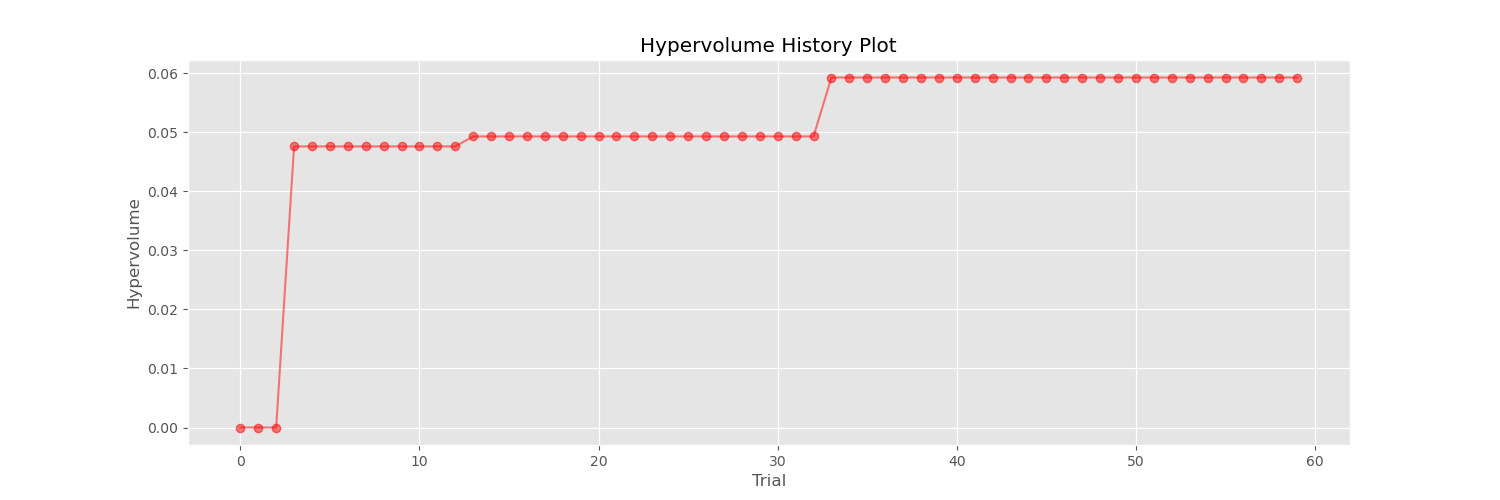
\includegraphics[width=1.0\textwidth]{./assets/images/hypervolume.png}
    \caption{Hypervolume history over optimization trials. The plot illustrates the convergence behavior of the NSGA-II algorithm, with hypervolume improving steadily and stabilizing around trial 35. This indicates a progressive exploration of the objective space and eventual convergence toward a robust Pareto-optimal solution.}
    \label{fig:hypervolume_history}
\end{figure}

\subsection{Observations}
\begin{figure}
    \centering
    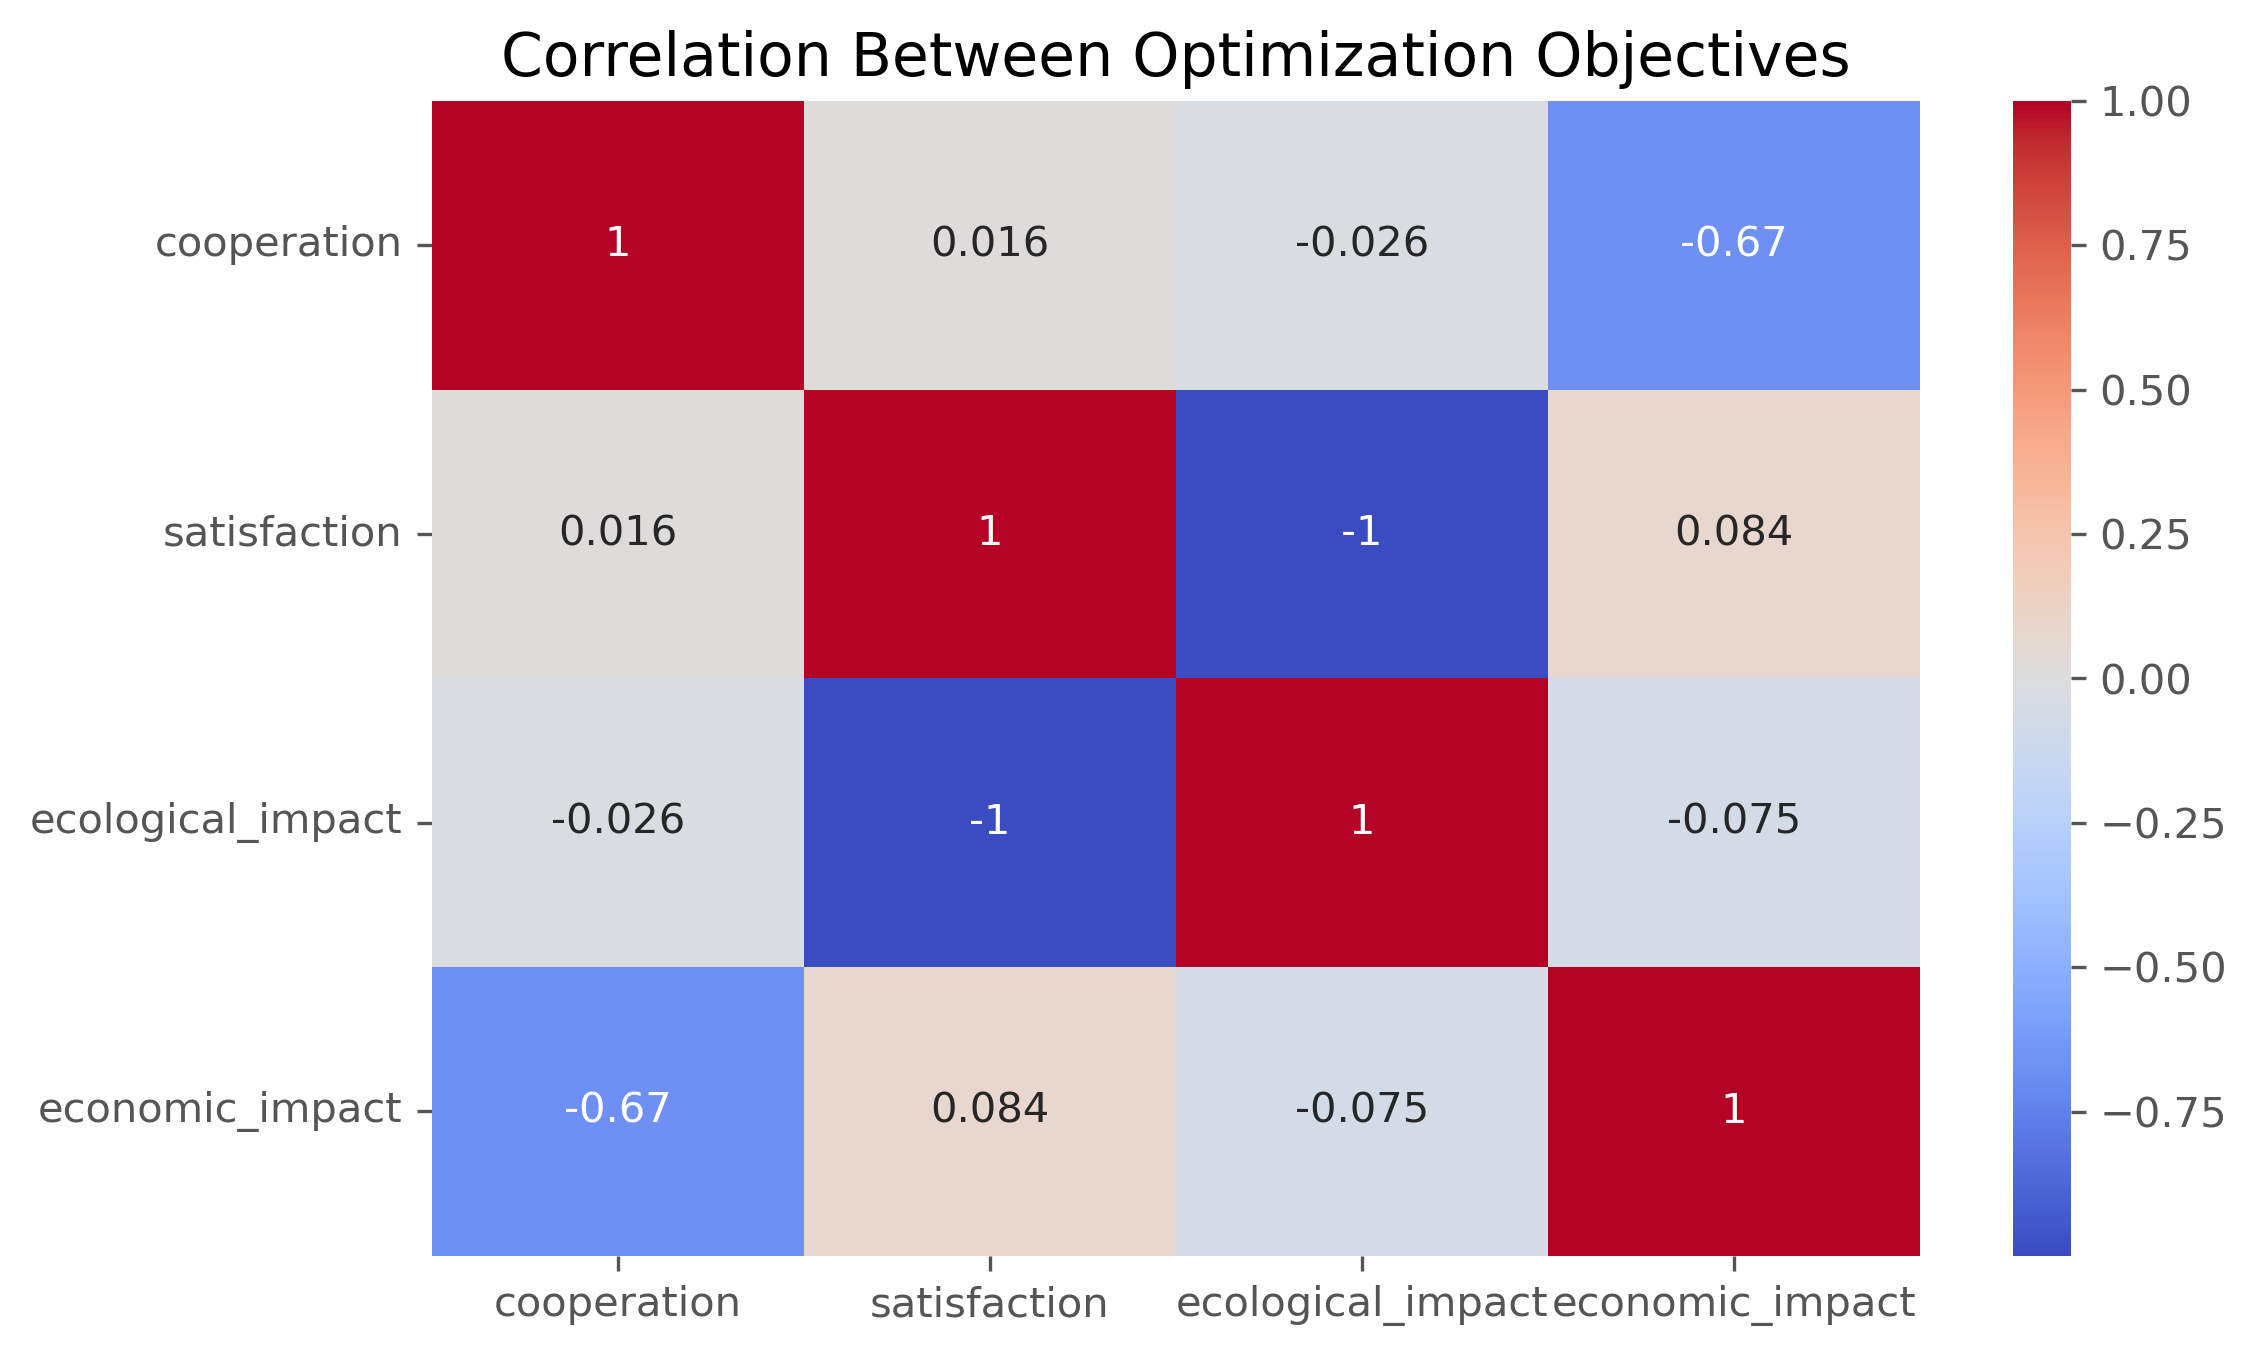
\includegraphics[width=0.7\textwidth]{./assets/images/objectives_correlation.png}
    \caption{Correlation matrix of optimization objectives. The plot highlights strong inverse relationships between key objectives, particularly between actor satisfaction and ecological impact ($r = -1.0$), and between cooperation and economic outcome ($r = -0.7$). These correlations underscore the inherent trade-offs in the multi-objective optimization landscape.}
    \label{fig:objectives_correlation}
\end{figure}

\begin{enumerate}

    \item \textbf{Satisfaction--Ecology Tradeoff}  
    
    A strong negative correlation ($r = -1.0$) was observed between actor satisfaction and ecological impact, indicating a near-perfect inverse relationship. Policies that maximize user satisfaction, particularly for high-priority actors, consistently result in elevated ecological stress, highlighting the fundamental tension between user demands and environmental preservation.

    \begin{itemize}
        \item Increasing water availability or allocation flexibility during scarcity events consistently improved satisfaction across actor types but led to higher ecological degradation.
        \item Emphasizing high-priority actor satisfaction skewed allocations, improving individual-level outcomes but intensifying overall environmental stress.
        \item Policies that constrained resource distribution in order to preserve ecological thresholds yielded the lowest satisfaction levels but were the most effective in limiting ecological impact.
        \item \textbf{Figure~\ref{fig:importance_satisfaction_ecology}} shows the hyperparameter importance plot. Priority weighting and crisis water thresholds emerge as the most influential parameters for this tradeoff, underscoring their central role in balancing satisfaction against ecological outcomes.
    \end{itemize}

    \item \textbf{Cooperation--Economy Link via Subvention}

    A moderately strong negative correlation ($r = -0.7$) was observed between economic outcomes and cooperation, particularly under subvention-heavy policy regimes. While subventions enhance individual actor incentives and promote cooperative behavior, they may also reduce systemic economic efficiency by encouraging resource redistribution over true productivity gains.

    \begin{itemize}
        \item Subventions increased cooperation by improving short-term actor returns, but they did not significantly raise total system economic output.
        \item Higher levels of cooperation under subsidy regimes often led to economic fragility and dependency, reducing long-term adaptability.
        \item Economic benefits were concentrated among actors best positioned to leverage subventions, raising concerns about equity and structural bias.
        \item \textbf{Figure~\ref{fig:importance_cooperation_economy}} illustrates that subvention-related hyperparameters are dominant drivers of cooperation. However, their marginal contribution to net economic outcomes highlights a potential misalignment in incentive structures.
    \end{itemize}

    \item \textbf{Diffusion of Cooperation Under Dissatisfaction}:  
    When satisfaction is achieved, cooperation levels tend to stabilize around a compact distribution—typically centered near 0.5—indicating a balanced and cohesive system. In contrast, low satisfaction scenarios produce more diffuse and variable cooperation, reflecting fragmentation that can destabilize system dynamics.  
    \begin{itemize}
        \item Medium-priority, high-demand actors tend to be less cooperative and more competitive during balanced cooperation-competition regimes. This arises because they occupy an intermediate position with limited buffer capacity and lower prioritization during scarcity.
        \item This dynamic is especially pronounced in the most ecologically sound solutions, where increased competition among high-demand actors plays a key role in system resilience.
    \end{itemize}

\noindent The $policy\_optimization$ notebook illustrates the difference in cooperation patterns between satisfied and unsatisfied regimes. The and $single\_scenario\_*$ demonstrate different single scenario outcomes for 
cooperation under satisfaction and dissatisfaction simulations.
\end{enumerate}

\begin{figure}[h]
    \centering
    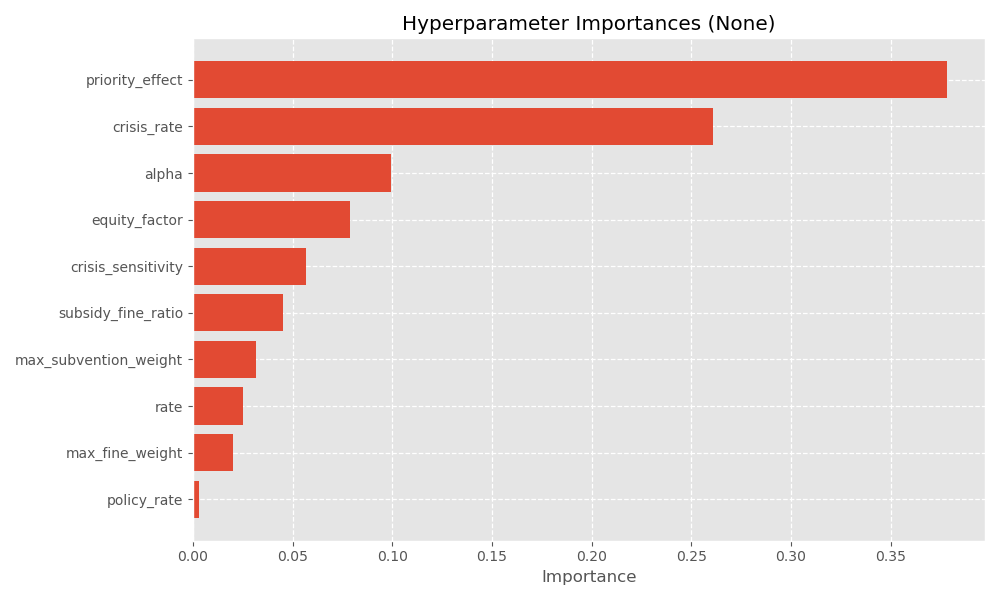
\includegraphics[width=0.7\textwidth]{./assets/images/optimization_hyp_importances_ecol.png}
    \caption{Hyperparameter importance for the Ecological Objectives. Priority weights and water availability thresholds are key drivers of the ecological health.}
    \label{fig:importance_satisfaction_ecology}
\end{figure}

\begin{figure}[h]
    \centering
    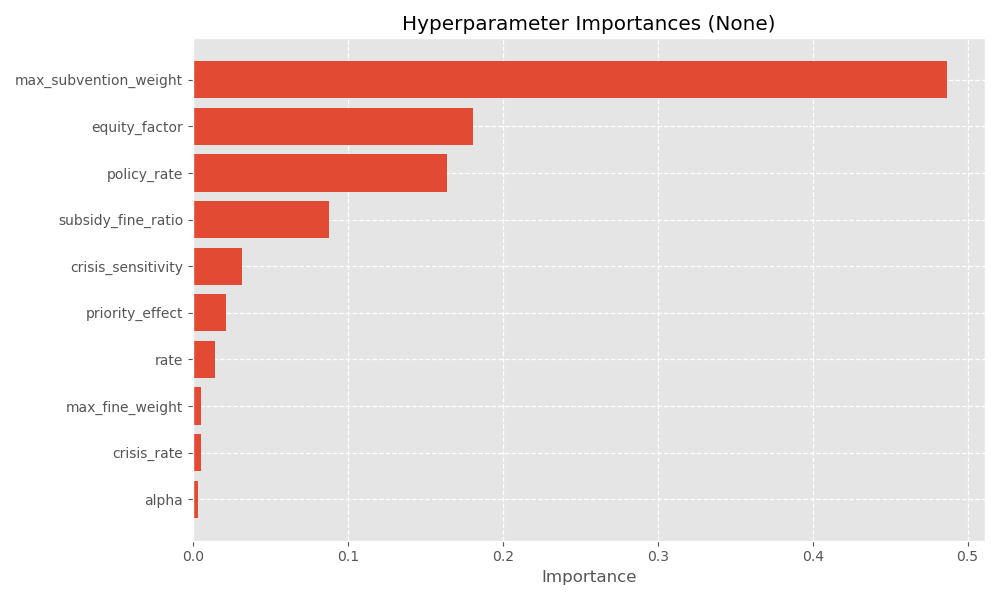
\includegraphics[width=0.7\textwidth]{./assets/images/optimization_hyp_importances_econ.png}
    \caption{Hyperparameter importance for cooperation and economic outcomes. Subvention levels and cooperation thresholds strongly influence cooperation, while their economic effects are more diffuse.}
    \label{fig:importance_cooperation_economy}
\end{figure}

\subsubsection{Post-Optimization Evaluation and Manual Selection}

Following the optimization, the final run of the NSGA-II algorithm yielded a single non-dominated solution on the Pareto front. Due to the lack of multiple trade-off candidates, we manually selected and evaluated additional promising trials—specifically Trial 33, Trial 46, and a configuration derived from the best parameters of the \texttt{pol\_regulator} policy.

These parameter sets were tested using the \texttt{multi\_scenario\_analysis} notebook to assess their performance across multiple objectives. To further refine outcomes, we manually adjusted some parameters to improve simulation results, focusing on satisfaction, economic impact, and ecological impact.

Table~\ref{tab:manual_vs_optimized} presents a comparison of the evaluated parameter sets. Trial 33 demonstrated the most favorable balance, achieving absolute satisfaction while maintaining acceptable ecological and economic trade-offs. Based on this analysis, Trial 33 was selected as the final solution for submission.

\begin{table}[h]
    \centering
    \begin{tabular}{l|c|c|c|c}
        % \toprule
        \textbf{Parameter Set} & \textbf{Satisfaction} & \textbf{Violations} & \textbf{Economic Impact} & \textbf{Ecological Impact} \\ \hline
        % \midrule
        Trial 33 (\textit{best})           & \textbf{1.000 }  & 0              & \textbf{0.885}                   & \textbf{0.935 }                    \\
        Trial 46                           & \textbf{1.000}   & 0              & 0.840                             & 0.941                     \\
        % \bottomrule
    \end{tabular}
    \caption{Comparison of parameter sets based on key optimization objectives}
    \label{tab:manual_vs_optimized}
\end{table}

\section{Conclusion and Future Work}
This work demonstrates a robust framework combining uncertainty-aware streamflow forecasting 
with multi-objective policy optimization, showing strong performance across spatiotemporal 
domains. Opportunities remain to improve efficiency and uncertainty handling. Future efforts 
will focus on optimizing model complexity for faster and more memory-efficient inference, 
enhancing uncertainty calibration to provide trustworthy prediction intervals across varied 
hydrological conditions, and developing transfer learning strategies to leverage knowledge 
from data-rich basins in underrepresented regions. Integrating real-time adaptation through 
online learning will further improve responsiveness to evolving data streams and environmental 
changes.\\

The policy optimization revealed fundamental trade-offs between actor satisfaction, ecological 
impact, cooperation, and economic outcomes. For example, a near-perfect negative correlation 
between satisfaction and ecological health underscores the challenge of balancing human needs 
with environmental sustainability. Cooperation improves with higher subvention levels but exhibits 
a negative correlation with economic performance, suggesting diminishing returns and potential 
long-term fragility. Behavioral analysis indicates that cooperation tends to concentrate around 
moderate levels when satisfaction is high, while dissatisfaction leads to fragmented patterns, 
highlighting system instability. Detailed single-scenario analyses validate these insights, 
reinforcing the importance of nuanced policy designs that balance competing objectives and 
leverage evolutionary optimization to identify effective solutions and meaningful system behaviors.
\begin{Backmatter}


\paragraph{Competing Interests}
None

\paragraph{Ethical Standards}
The research meets all ethical guidelines, including adherence to the legal requirements of the study country.

\paragraph{Author Contributions}
Conceptualization: D.A.; Methodology: D.A; Data curation: D.A. Data visualisation: D.A. Writing original draft: D.A; All authors approved the final submitted draft.

\begin{thebibliography}{}

\bibitem[Beven, 2012]{beven2012rainfall}
\textbf{Beven, KJ} (2012) \emph{Rainfall-Runoff Modelling: The Primer}. \textit{Chichester: Wiley-Blackwell}.

\bibitem[Singh, 1995]{singh1995}
\textbf{Singh VP} (1995) Computer Models of Watershed Hydrology, \textit{Water Resources Publications}

\bibitem[Mosavi et al., 2018]{mosavi2018}
\textbf{Mosavi A, Ozturk P, and Chau KW} (2018) Flood prediction using machine learning models: A review, \textit{Water} \textit{10}(11), {1536}.

\bibitem[Kratzert et al., 2019]{kratzert2019}
\textbf{Kratzert F, Klotz D, Brenner C, Schulz K, and Herrnegger M} (2019) Neural Hydrology: Interpreting LSTMs in Hydrology, \textit{Hydrology and Earth System Sciences} \textit{23} {375}–--{397}.

\bibitem[Prokhorenkova et al., 2018]{prokhorenkova2018}
\textbf{Prokhorenkova L, Gusev G, Vorobev A, Dorogush A, and Gulin A} (2018) CatBoost: unbiased boosting with categorical features, \textit{Advances in Neural Information Processing Systems} \textit{31}.

\bibitem[Spyromitros et al., 2016]{spyromitros2016}
\textbf{Spyromitros-Xioufis E, Tsoumakas G, Groves W, and Vlahavas I} (2016) Multi-target regression via input space expansion: Treating targets as inputs, \textit{European Conference on Machine Learning and Principles and Practice of Knowledge Discovery in Databases} {105}--–{120} {Springer}

\bibitem[Romano et al., 2019]{romano2019}
\textbf{Romano Y, Patterson E, and Candes EJ} (2019) Conformalized quantile regression, \textit{Advances in Neural Information Processing Systems} \textit{32}.

\bibitem[Angelopoulos and Bates, 2022]{angebates2022}
\textbf{Angelopoulos A and Bates S} (2022) A gentle introduction to conformal prediction and distribution-free uncertainty quantification, \textit{arXiv e-prints} \textit{Art. no. arXiv:2107.07511v6, 2022. doi:10.48550/arXiv.2107.07511}

\bibitem[Sousa et al., 2022]{sousa2022}
\textbf{Sousa M, Tomé AM, and Moreira J} (2022) Improved conformalized quantile regression, \textit{arXiv e-prints} \textit{Art. no. arXiv:2207.02808, 2022. doi:10.48550/arXiv.2207.02808}

\bibitem[Hort et al., 2024 ]{hjort2024}
\textbf{Hjort A, Williams JP, and Pensar J} (2024) Clustered Conformal Prediction for the Housing Market, \textit{Proceedings of the Thirteenth Symposium on Conformal and Probabilistic Prediction with Applications}, \textit{Proceedings of Machine Learning Research PMLR} 230:366-386, Available from https://proceedings.mlr.press/v230/hjort24a.html.

\bibitem[Ding et al., 2023]{ding2023}
\textbf{Ding T, Angelopoulos AN, Bates S, Jordan M, and Tibshirani R} (2023) Class-Conditional Conformal Prediction with Many Classes, \textit{Thirty-seventh Conference on Neural Information Processing Systems}, Available from https://openreview.net/forum?id=mYz6ApeU4J.

\bibitem[Marx et al., 2022]{marx2022}
\textbf{Marx C, Zhao S, Neiswanger W, and Ermon S} (2022). Modular Conformal Calibration, \textit{Proceedings of the 39th International Conference on Machine Learning (ICML)} Available at: https://arxiv.org/abs/2206.11468

\bibitem[Deutsmann et al., 2023]{deutschmann2023}
\textbf{Deutschmann N, Rigotti M, and Rodríguez Martínez M} (2023) Adaptive Conformal Regression with Jackknife+ Rescaled Scores, \textit{arXiv preprint arXiv:2305.19901}, Available at: https://arxiv.org/abs/2305.19901

\bibitem[Arsenault et al., 2023]{arsenault2023}
\textbf{Arsenault R, Martel J-L, Brunet F, Brissette F, and Mai J} (2023) Continuous streamflow Prediction in Ungauged Basins: Long Short-Term Memory in Neural Networks Clearly Outperform Traditional Hydrological Models, \textit{Hydrology and Earth System Sciences}, \textit{27}(1), 139–157, \textit{https://hess.copernicus.org/articles/27/139/2023/hess-27-139-2023.pdf}

\bibitem[Kuhn and Johnson(2019)]{kuhnjohnson2019} 
\textbf{Kuhn M and Johnson K} (2019). \textit{Feature Engineering and Selection: A Practical Approach for Predictive Models}. \textit{Chapman and Hall/CRC}.

\bibitem[Hyndman and Athanasopolous, 2018]{hyndman2018}
\textbf{Hyndman R and Athanasopolous G} (2018). \textit{Forecasting: Principles and Practice}. \textit{OTexts}.

\bibitem[Peng, 2005]{peng2005}
\textbf{Peng H} (2005)Feature Selection Based on Mutual Information: Criteria of Max-Dependency, Max-Relevance, and Min-Redundancy. \textit{IEEE Transactions on Pattern Analysis and Machine Intelligence}, \textit{27}(8):1226-1238, \textit{doi:10.1109/TPAMI.2005.159}

\bibitem[Shortridge et al., 2016]{shortridge2016}
\textbf{Shortridge JE, Guikema SD, Zaitchik BF.} (2016) Machine Learning Methods for Empirical Streamflow Simulation: A comparison of Model Accuracy. \textit{Hydrological Processes}, 30(3): 366-376. DOI: 10.1002/hyp.10573

\bibitem[Kumar et al., 2023]{kumar2023}
\textbf{Kumar V, Kedam N, Sharma KV, Mehta DJ, and Caloiero T} (2023) Advanced Machine Learning Techniques to Improve Hydrological Prediction: A Comparative Analysis of Streamflow Prediction Models, \textit{Water}, \textit{15}(14):2572, \textit{https://doi.org/10.3390/w15142572}

\bibitem[Stephens, 2000]{stephen2000}
\textbf{Stephens M} (2000) Dealing with Label Switching in Mixture Models, \textit{Journal of the Royal Statistical Society: Series B}, \textit{62}(4): 795-809.

\bibitem[Strehl et al., 2003]{strehl2003}
\textbf{Strehl A and Ghosh J} (2003) Cluster Ensembles - A Knowledge Reuse Framework for Combining Multiple Partitions, \textit{Journal of Machine Learning Research}, \textit{3}: 583-617.

\bibitem[Kuhn, 1955]{kuhn1955}
\textbf{Kuhn HW} (1955) The Hungarian Method for the Assignment Problem, \textit{Naval Research Logistics Quarterly}, \textit{2}(1-2): 83-97.

\bibitem[Wang, 2025]{wang2025}
\textbf{Wang X} (2025) Sustainable Water Management: Balancing Social, Economic, and Environmental Needs. \textit{Journal of Lifestyle and SDG Reviews}, \textit{5}(5) e06606 \textit{https://doi.org/10.47172/2965-730X.SDGsReview.v5.n05.pe06606}

\bibitem[Tian et al., 2019][tian2019]
\textbf{Tian J, Guo S, Liu D, Pan Z, and Hong X} (2019) A Fair Approach for Multi-Objective Water Resources Allocation, \textit{Water Resources Management}, \textit{33}, 3633-3653 \textit{https://doi.org/10.1007/s11269-019-02323-5}

\bibitem[Tang et al., 2021]{tang2021}
\textbf{Tang X, He Y, Qi P, Chang Z, Jiang M and Dai Z} (2021) A New Multi-Objective Optimization Model of Water Resources Considering Fairness and Water Shortage Risk, \textit{Water}, \textit{13}, 2648, \textit{https://doi.org/10.3390/w13192648}

\bibitem[Fu et al., 2020]{fu2020}
\textbf{Fu Q, Li L, Li M, Li T, Liu D, and Cui S} (2018) A Simulation-Based Linear Fractional Programming Model for Adaptable Water Allocation Planning in the Main Stream of the Songhua River Basin, China, \textit{Water}, \textit{10}(5), 627, \textit{https://doi.org/10.3390/w10050627}

\end{thebibliography}
\end{Backmatter}
\end{document}
